% MIT License
%
% Copyright (c) 2018 José Nascimento <joseaugustodearaujonascimento@gmail.com>
%
% Permission is hereby granted, free of charge, to any person obtaining a copy
% of this software and associated documentation files (the "Software"), to deal
% in the Software without restriction, including without limitation the rights
% to use, copy, modify, merge, publish, distribute, sublicense, and/or sell
% copies of the Software, and to permit persons to whom the Software is
% furnished to do so, subject to the following conditions:
%
% The above copyright notice and this permission notice shall be included in all
% copies or substantial portions of the Software.
%
% THE SOFTWARE IS PROVIDED "AS IS", WITHOUT WARRANTY OF ANY KIND, EXPRESS OR
% IMPLIED, INCLUDING BUT NOT LIMITED TO THE WARRANTIES OF MERCHANTABILITY,
% FITNESS FOR A PARTICULAR PURPOSE AND NONINFRINGEMENT. IN NO EVENT SHALL THE
% AUTHORS OR COPYRIGHT HOLDERS BE LIABLE FOR ANY CLAIM, DAMAGES OR OTHER
% LIABILITY, WHETHER IN AN ACTION OF CONTRACT, TORT OR OTHERWISE, ARISING FROM,
% OUT OF OR IN CONNECTION WITH THE SOFTWARE OR THE USE OR OTHER DEALINGS IN THE
% SOFTWARE.
\documentclass[
  % -- opções da classe memoir --
  12pt,                 % tamanho da fonte
  openright,            % capítulos começam em pág ímpar (insere página vazia caso preciso)
  oneside,              % para impressão em recto e verso. Oposto a oneside
  a4paper,              % tamanho do papel.
  % -- opções da classe abntex2 --
  sumario=abnt-6027-2012,
  chapter=TITLE,        % títulos de capítulos convertidos em letras maiúsculas
  section=TITLE,        % títulos de seções convertidos em letras maiúsculas
  %subsection=TITLE,    % títulos de subseções convertidos em letras maiúsculas
  %subsubsection=TITLE, % títulos de subsubseções convertidos em letras maiúsculas
  % -- opções do pacote babel --
  english,              % idioma adicional para hifenização
  french,               % idioma adicional para hifenização
  spanish,              % idioma adicional para hifenização
  brazil                % o último idioma é o principal do documento
]{abntex2}

% ---
% Pacotes básicos
% ---

\usepackage{lmodern}        % Usa a fonte Latin Modern
\usepackage{times}          % Usa a fonte Times New Roman
\usepackage[T1]{fontenc}    % Selecao de codigos de fonte.
\usepackage[utf8]{inputenx} % Codificacao do documento (conversão automática dos acentos)
\usepackage{indentfirst}    % Indenta o primeiro parágrafo de cada seção.
\usepackage{color}          % Controle das cores
\usepackage{graphicx}       % Inclusão de gráficos
\usepackage{microtype}      % para melhorias de justificação
% ---

% ---
% Pacotes de citações
% ---
\usepackage[brazilian,hyperpageref]{backref}   % Paginas com as citações na bibl
\usepackage[alf,abnt-emphasize=bf]{abntex2cite}  % Citações padrão ABNT

% ---
% CONFIGURAÇÕES DE PACOTES
% ---

% ---
% Configurações do pacote backref
% Usado sem a opção hyperpageref de backref
%\renewcommand{\backrefpagesname}{Citado na(s) página(s):~}
\renewcommand{\backrefpagesname}{}
% Texto padrão antes do número das páginas
\renewcommand{\backref}{}
% Define os textos da citação
% \renewcommand*{\backrefalt}[4]{
%   \ifcase #1 %
%     Nenhuma citação no texto.%
%   \or
%     Citado na página #2.%
%   \else
%     Citado #1 vezes nas páginas #2.%
%   \fi}%
\renewcommand*{\backrefalt}[4]{}
% ---

\usepackage{textcase}
\usepackage[useregional]{datetime2}
\usepackage{datetime2-calc}
\usepackage[normalem]{ulem}

\usepackage[hypcap=true,justification=centering,skip=0cm]{caption}
\usepackage[justification=centering,skip=0cm]{subcaption}

% \usepackage{newpxtext}
\captionsetup[table]{skip=0cm}
\captionsetup[figure]{skip=0cm}
\captionsetup[subfigure]{skip=0cm}

\usepackage{hyphenat}
\usepackage{booktabs}
\usepackage{navigator}
\usepackage{listings}

% \usepackage{float}
\usepackage{multirow}
% \usepackage[all]{nowidow}

\usepackage{mdframed}

% \setfloatlocations{figure}{!htb}
\setfloatlocations{figure}{!hbtp}
\setfloatlocations{table}{!hbtp}

\graphicspath{ {./imagens/} }

\usepackage{enumitem}
% \setlist{itemsep=4pt,parsep=4pt,topsep=8pt,partopsep=4pt}
% \setlist{nosep}

% \floatstyle{boxed}
% \restylefloat{figure}

\usepackage[dvipsnames]{xcolor}

\definecolor{tamarillo}{RGB}{163,20,20}
\definecolor{brightturquoise}{rgb}{0.03, 0.91, 0.87}
\definecolor{malachite}{rgb}{0.04, 0.85, 0.32}

% Redefinição de instruções

\providecommand{\tightlist}{%
  \setlength{\itemsep}{0pt}\setlength{\parskip}{0pt}
}

% \renewcommand{\listingscaption}{Fig.}
% \renewcommand\theFancyVerbLine{\rm{\arabic{FancyVerbLine}}}

% -----
% Declarações de cabecalhos
% -----
% Cabecalho padrao
\makepagestyle{abntbookheadings}
% \makeevenhead{abntbookheadings}{\ABNTEXfontereduzida\thepage}{}{}
\makeevenhead{abntbookheadings}{}{}{\ABNTEXfontereduzida\thepage}
\makeoddhead{abntbookheadings}{}{}{\ABNTEXfontereduzida\thepage}
%\makeheadrule{abntbookheadings}{\textwidth}{\normalrulethickness}

% Cabecalho do inicio do capitulo
\makepagestyle{abntbookchapfirst}
\makeoddhead{abntbookchapfirst}{}{}{\ABNTEXfontereduzida\thepage}

% Configura layout para elementos textuais
\renewcommand{\textual}{%
  \pagestyle{abntbookheadings}%
  \aliaspagestyle{chapter}{abntbookchapfirst}% customizing chapter pagestyle
  %\nouppercaseheads%
  \bookmarksetup{startatroot}%
}
% ---

\DTMsavedate{mdate}{2018-06-11}
\date{\DTMusedate{mdate}}

\title{EVA: Desenvolvimento de um Chatbot para a Escola Virtual de Governo}
\author{Mauro de Carvalho Gonçalves}
\local{\uppercase{Natal-RN}}
\date{2018}
\orientador{Leonardo Ataide Minora}
\instituicao{%
  Instituto Federal do Rio Grande do Norte -- IFRN
  \par
  Diretoria de Gestão e Tecnologia da Informação -- DIATINF
  \par
  Curso de Tecnologia em Análise e Desenvolvimento de Sistemas -- TADS
}
\tipotrabalho{TCC (Graduação)}
% O preambulo deve conter o tipo do trabalho, o objetivo,
% o nome da instituição e a área de concentração
\preambulo{%
Trabalho de conclusão de curso apresentado ao Curso Superior de Tecnologia em Análise e Desenvolvimento de Sistemas da Diretoria de Gestão e Tecnologia da Informação do Instituto Federal de Educação, Ciência e Tecnologia do Rio Grande do Norte como requisito parcial à obtenção do título de Tecnólogo em Análise e Desenvolvimento de Sistemas.
}

\makeatletter
\hypersetup{
  pdftitle={\@title},
  pdfauthor={\@author},
  pdfsubject={\imprimirpreambulo},
  pdfkeywords={PALAVRAS}{CHAVE}{EM}{PORTUGUES},
  pdfcreator={LaTeX with abnTeX2},
  colorlinks=false,
  linkcolor=blue,
  citecolor=blue,
  urlcolor=blue
}
\makeatother

% ---
% Possibilita criação de Quadros e Lista de quadros.
% Ver https://github.com/abntex/abntex2/issues/176
%
\newcommand{\quadroname}{Quadro}
\newcommand{\listofquadrosname}{Lista de quadros}

\newfloat{quadro}{loq}{\quadroname}
\newlistof{listofquadros}{loq}{\listofquadrosname}
\newlistentry{quadro}{loq}{0}

% configurações para atender às regras da ABNT
\setfloatadjustment{quadro}{\centering}
\counterwithout{quadro}{chapter}
\renewcommand{\cftquadroname}{\quadroname\space} 
\renewcommand*{\cftquadroaftersnum}{\hfill--\hfill}

\setfloatlocations{quadro}{!hbtp}

\makeatletter
\renewcommand*{\ext@quadro}{lof}
\makeatother
% ---

% ---
% Posiciona figuras e tabelas no topo da página quando adicionadas sozinhas
% em um página em branco. Ver https://github.com/abntex/abntex2/issues/170
\makeatletter
\setlength{\@fptop}{5pt} % Set distance from top of page to first float
\makeatother
% ---

\renewcommand{\fontename}{Fonte}
\renewcommand{\ABNTEXcaptionfontedelim}{:}

\makeatletter
\renewcommand{\fonte}[2][\fontename]{%
  \memlegendinfo{#2}%
  \par
\begingroup
    \ABNTEXfontereduzida
    \configureseparator
    \captiondelim{:~}
    \@makecaption{\ABNTEXfontereduzida #1}{\ignorespaces\ABNTEXfontereduzida #2}\par
\endgroup}
\makeatother

\newcommand{\mfonte}[0]{%
  \fonte{Elaboração própria em \DTMfetchyear{mdate}}}

\newcommand{\mcaption}[1]
{%
  \caption[#1]{%
    #1
  }
}

\newcommand{\alusao}[1]{\citeauthor{#1}~(\citeyear{#1})}

\mdfsetup{
  leftmargin=0cm,
  skipabove=0cm,
  rightmargin=0cm,
  skipbelow=0cm,
  innertopmargin=.1cm,
  innerrightmargin=.1cm,
  innerleftmargin=.1cm,
  innerbottommargin=.1cm,
}

\newlength{\MaxSizeOfLineNumbers}%
% Adjust to maximum number of lines
\settowidth{\MaxSizeOfLineNumbers}{99}%
\addtolength{\MaxSizeOfLineNumbers}{2.5ex}%
\lstset{
  showstringspaces=false,
  numbers=left,
  numbersep=2.5ex,
  xleftmargin=\MaxSizeOfLineNumbers,
  keywordstyle=\color{blue},
  basicstyle=\ttfamily,
  breaklines=true,
  stringstyle=\color{tamarillo},
  literate=
    {á}{{\'a}}1
    {à}{{\`a}}1
    {é}{{\'e}}1
    {ê}{{\^e}}1
    {ã}{{\~a}}1
    {ó}{{\'o}}1
    {ç}{{\c{c}}}1%
}
\renewcommand\sout[1]{}
\usepackage[export]{adjustbox}

\let\oldincludegraphics\includegraphics
\renewcommand{\includegraphics}[2][]{%
%   \begin{mdframed}%
%   \begin{center}%
    \centering%
    \oldincludegraphics[max width=.7\linewidth,#1]{#2}%
%   \end{center}%
%   \end{mdframed}%
}

\setlength{\ABNTEXsignwidth}{10cm}

% ---
% Espaçamentos entre linhas e parágrafos
% ---

% O tamanho do parágrafo é dado por:
\setlength{\parindent}{1.3cm}

% Controle do espaçamento entre um parágrafo e outro:
\setlength{\parskip}{0.2cm}  % tente também \onelineskip

% \renewcommand{\ABNTEXchapterfont}{\bfseries}
% \newcommand{\ABNTEXpartfont}{\ABNTEXchapterfont}
%
% Fontes das entradas do sumario
%
% \renewcommand{\cftpartfont}{\bfseries\larger}

\renewcommand*{\cftchapterleader}{\hfill}
\renewcommand*{\cftsectionleader}{\hfill}
\renewcommand*{\cftsubsectionleader}{\hfill}
\renewcommand*{\cftsubsubsectionleader}{\hfill}
\renewcommand*{\cftparagraphleader}{\hfill}

\setlength{\cftbeforechapterskip}{0em}

%--
% seção primária
%--
\renewcommand{\cftchapterfont}{\bfseries}
\renewcommand{\cftchapterpagefont}{\normalsize\normalfont}
%--
% seção secundária
%--
\renewcommand{\cftsectionfont}{\normalfont}
\renewcommand{\cftsectionpagefont}{\normalsize\normalfont}
%--
% seção terciária
%--
\renewcommand{\cftsubsectionfont}{\normalfont\bfseries}
\renewcommand{\cftsubsectionpagefont}{\normalsize\normalfont}
%--
% seção quaternária
%--
\renewcommand{\cftsubsubsectionfont}{\normalfont}
\renewcommand{\cftsubsubsectionpagefont}{\normalsize\normalfont}
%--
% seção quinária
%--
\renewcommand{\cftparagraphfont}{\normalfont\itshape}
\renewcommand{\cftparagraphpagefont}{\normalsize\normalfont}

\makeatletter
\let\oldcontentsline\contentsline
\def\contentsline#1#2{%
  \expandafter\ifx\csname l@#1\endcsname\l@section
  \expandafter\@firstoftwo
  \else
  \expandafter\@secondoftwo
  \fi
  {%
    \oldcontentsline{#1}{\MakeTextUppercase{#2}}%
  }{%
  \oldcontentsline{#1}{#2}%
}%
}
\makeatother

% \renewcommand{\cftsubsectionfont}{\bfseries}
% \renewcommand{\cftsubsectionpagefont}{\normalsize\cftsubsectionfont}

% \renewcommand{\cftsubsubsectionfont}{\normalsize}
% \renewcommand{\cftsubsubsectionpagefont}{\cftsubsubsectionfont}

% \renewcommand{\cftparagraphfont}{\footnotesize}
% \renewcommand{\cftparagraphpagefont}{\cftparagraphfont}

%
% Fontes das seções/capítulos
%
\renewcommand{\ABNTEXpartfontsize}{\normalsize}

\renewcommand{\ABNTEXchapterfont}{\bfseries}
\renewcommand{\ABNTEXchapterfontsize}{\normalsize}

\renewcommand{\ABNTEXsectionfont}{\normalsize}
\renewcommand{\ABNTEXsectionfontsize}{\normalsize}

\renewcommand{\ABNTEXsubsectionfont}{\bfseries}
\renewcommand{\ABNTEXsubsectionfontsize}{\normalsize}

\renewcommand{\ABNTEXsubsubsectionfontsize}{\normalfont}
\renewcommand{\ABNTEXsubsubsubsectionfontsize}{\normalfont\itshape}

% \newcommand{\ABNTEXsectionfont}{\ABNTEXchapterfont}
% \newcommand{\ABNTEXsubsectionfont}{\ABNTEXsectionfont}
% \newcommand{\ABNTEXsubsubsectionfont}{\ABNTEXsubsectionfont}
% \newcommand{\ABNTEXsubsubsubsectionfont}{\ABNTEXsubsectionfont}

% ---
% compila o indice
% ---
\makeindex

% \setlength{\parindent}{1pt}
\setlength{\parskip}{0pt}

\setlength{\beforechapskip}{1.0\onelineskip}
\setlength{\afterchapskip}{1.0\onelineskip}

\setlength{\beforesecskip}{1.0\onelineskip}
\setlength{\aftersecskip}{1.0\onelineskip}

\setlength{\beforesubsecskip}{1.0\onelineskip}
\setlength{\aftersubsecskip}{1.0\onelineskip}

\setlength{\textfloatsep}{1.0\onelineskip}
\setlength{\floatsep}{1.0\onelineskip}
\setlength{\intextsep}{1.0\onelineskip}

% \setlength{\abovecaptionskip}{0pt}
% \setlength{\belowcaptionskip}{0pt}

% \renewcommand\cleardoublepage{}

% Inicio do documento
\begin{document}
  \selectlanguage{brazil}
  \frenchspacing

  \frontmatter

  % MIT License
%
% Copyright (c) 2018 José Nascimento <joseaugustodearaujonascimento@gmail.com>
%
% Permission is hereby granted, free of charge, to any person obtaining a copy
% of this software and associated documentation files (the "Software"), to deal
% in the Software without restriction, including without limitation the rights
% to use, copy, modify, merge, publish, distribute, sublicense, and/or sell
% copies of the Software, and to permit persons to whom the Software is
% furnished to do so, subject to the following conditions:
%
% The above copyright notice and this permission notice shall be included in all
% copies or substantial portions of the Software.
%
% THE SOFTWARE IS PROVIDED "AS IS", WITHOUT WARRANTY OF ANY KIND, EXPRESS OR
% IMPLIED, INCLUDING BUT NOT LIMITED TO THE WARRANTIES OF MERCHANTABILITY,
% FITNESS FOR A PARTICULAR PURPOSE AND NONINFRINGEMENT. IN NO EVENT SHALL THE
% AUTHORS OR COPYRIGHT HOLDERS BE LIABLE FOR ANY CLAIM, DAMAGES OR OTHER
% LIABILITY, WHETHER IN AN ACTION OF CONTRACT, TORT OR OTHERWISE, ARISING FROM,
% OUT OF OR IN CONNECTION WITH THE SOFTWARE OR THE USE OR OTHER DEALINGS IN THE
% SOFTWARE.

\begin{capa}
  \begin{center}

    \begin{SingleSpacing}%
      \uppercase{%
        INSTITUTO FEDERAL DE EDUCAÇÃO, CIÊNCIA E TECNOLOGIA\\
        DO RIO GRANDE DO NORTE
        \par
      }%
    \end{SingleSpacing}%

    \vspace*{\fill}

    \begin{center}
      \MakeUppercase{\imprimirautor}
    \end{center}

    \vspace*{\fill}

    % Nome do aluno (autor)
    \MakeUppercase{\imprimirtitulo}

    \vspace*{\fill}\vspace*{\fill}
    \vspace*{\fill}

    \imprimirlocal{}\\
    \imprimirdata
    \par
  \end{center}
\end{capa}
%--
  % MIT License
%
% Copyright (c) 2018 José Nascimento <joseaugustodearaujonascimento@gmail.com>
%
% Permission is hereby granted, free of charge, to any person obtaining a copy
% of this software and associated documentation files (the "Software"), to deal
% in the Software without restriction, including without limitation the rights
% to use, copy, modify, merge, publish, distribute, sublicense, and/or sell
% copies of the Software, and to permit persons to whom the Software is
% furnished to do so, subject to the following conditions:
%
% The above copyright notice and this permission notice shall be included in all
% copies or substantial portions of the Software.
%
% THE SOFTWARE IS PROVIDED "AS IS", WITHOUT WARRANTY OF ANY KIND, EXPRESS OR
% IMPLIED, INCLUDING BUT NOT LIMITED TO THE WARRANTIES OF MERCHANTABILITY,
% FITNESS FOR A PARTICULAR PURPOSE AND NONINFRINGEMENT. IN NO EVENT SHALL THE
% AUTHORS OR COPYRIGHT HOLDERS BE LIABLE FOR ANY CLAIM, DAMAGES OR OTHER
% LIABILITY, WHETHER IN AN ACTION OF CONTRACT, TORT OR OTHERWISE, ARISING FROM,
% OUT OF OR IN CONNECTION WITH THE SOFTWARE OR THE USE OR OTHER DEALINGS IN THE
% SOFTWARE.

\begin{folhaderosto}
%\imprimirfolhaderosto{}

  \begin{center}
    \MakeUppercase{\imprimirautor}

    \vspace*{\fill}\vspace*{\fill}
    \begin{center}
      \MakeUppercase{\imprimirtitulo}
    \end{center}
    \vspace*{\fill}\vspace*{\fill}
  \end{center}

  %\vspace*{\fill}

  \hspace*{\fill}
  \begin{minipage}{.5\textwidth}
    \SingleSpace
    \imprimirpreambulo
    \\[\baselineskip]
    Orientador: M.e \imprimirorientador
  \end{minipage}

  \vspace*{\fill}\vspace*{\fill}
  \vspace*{\fill}\vspace*{\fill}
  \vspace*{\fill}\vspace*{\fill}
  \vspace*{\fill}\vspace*{\fill}

  \begin{center}
      \imprimirlocal{}\\
      \imprimirdata
      \par
  \end{center}

\end{folhaderosto}
%--

  % MIT License
%
% Copyright (c) 2018 José Nascimento <joseaugustodearaujonascimento@gmail.com>
%
% Permission is hereby granted, free of charge, to any person obtaining a copy
% of this software and associated documentation files (the "Software"), to deal
% in the Software without restriction, including without limitation the rights
% to use, copy, modify, merge, publish, distribute, sublicense, and/or sell
% copies of the Software, and to permit persons to whom the Software is
% furnished to do so, subject to the following conditions:
%
% The above copyright notice and this permission notice shall be included in all
% copies or substantial portions of the Software.
%
% THE SOFTWARE IS PROVIDED "AS IS", WITHOUT WARRANTY OF ANY KIND, EXPRESS OR
% IMPLIED, INCLUDING BUT NOT LIMITED TO THE WARRANTIES OF MERCHANTABILITY,
% FITNESS FOR A PARTICULAR PURPOSE AND NONINFRINGEMENT. IN NO EVENT SHALL THE
% AUTHORS OR COPYRIGHT HOLDERS BE LIABLE FOR ANY CLAIM, DAMAGES OR OTHER
% LIABILITY, WHETHER IN AN ACTION OF CONTRACT, TORT OR OTHERWISE, ARISING FROM,
% OUT OF OR IN CONNECTION WITH THE SOFTWARE OR THE USE OR OTHER DEALINGS IN THE
% SOFTWARE.

\begin{folhadeaprovacao}
  \OnehalfSpacing

  \begin{center}
    \MakeUppercase{\imprimirautor}

    \vspace*{\fill}\vspace*{\fill}
    \begin{center}
      \MakeUppercase{\imprimirtitulo}
    \end{center}
    \vspace*{\fill}
  \end{center}

  {
    \hspace*{\fill}
    \begin{minipage}{.5\textwidth}%
      \SingleSpacing
      \imprimirpreambulo%
    \end{minipage}%
  }
    \vspace*{\fill}
    \vspace*{\fill}
    \vspace*{\fill}

Trabalho de Conclusão de Curso apresentado e aprovado em \_\_\_/\_\_\_/\_\_\_\_, pela seguinte Banca Examinadora:

  \centering
    \begin{center}%
      BANCA EXAMINADORA
    \end{center}%

    \assinatura{
      \imprimirorientador, M.e -- Presidente\\
      Instituto Federal de Educação, Ciência e Tecnologia do Rio Grande do Norte
    }

    \assinatura{
      José Antônio da Cunha, M.e -- Examinador\\
      Instituto Federal de Educação, Ciência e Tecnologia do Rio Grande do Norte
    }

    \assinatura{
      Bruno Pereira Pontes -- Examinador\\
      Instituto Federal de Educação, Ciência e Tecnologia do Rio Grande do Norte
    }

  \vspace*{\fill}
  \begin{center}
    \begin{SingleSpacing}
      \imprimirlocal{}\\
      \imprimirdata
    \end{SingleSpacing}
  \end{center}

\end{folhadeaprovacao}
%---
  % MIT License
%
% Copyright (c) 2018 José Nascimento <joseaugustodearaujonascimento@gmail.com>
%
% Permission is hereby granted, free of charge, to any person obtaining a copy
% of this software and associated documentation files (the "Software"), to deal
% in the Software without restriction, including without limitation the rights
% to use, copy, modify, merge, publish, distribute, sublicense, and/or sell
% copies of the Software, and to permit persons to whom the Software is
% furnished to do so, subject to the following conditions:
%
% The above copyright notice and this permission notice shall be included in all
% copies or substantial portions of the Software.
%
% THE SOFTWARE IS PROVIDED "AS IS", WITHOUT WARRANTY OF ANY KIND, EXPRESS OR
% IMPLIED, INCLUDING BUT NOT LIMITED TO THE WARRANTIES OF MERCHANTABILITY,
% FITNESS FOR A PARTICULAR PURPOSE AND NONINFRINGEMENT. IN NO EVENT SHALL THE
% AUTHORS OR COPYRIGHT HOLDERS BE LIABLE FOR ANY CLAIM, DAMAGES OR OTHER
% LIABILITY, WHETHER IN AN ACTION OF CONTRACT, TORT OR OTHERWISE, ARISING FROM,
% OUT OF OR IN CONNECTION WITH THE SOFTWARE OR THE USE OR OTHER DEALINGS IN THE
% SOFTWARE.

\begin{dedicatoria}
\vspace*{\fill}
\begingroup
\leftskip=4cm
\noindent%
Dedico esse trabalho à minha avó, Lauricy Luz, e ao meu pai, Márcio Jeferson, com todo meu amor e gratidão, por tudo que fizeram por mim ao longo de minha vida. Desejo poder ter sido merecedor do esforço dedicado por vocês em todos os aspectos, especialmente quanto à minha formação.%
\par
\endgroup
\end{dedicatoria}
%--

  % MIT License
%
% Copyright (c) 2018 José Nascimento <joseaugustodearaujonascimento@gmail.com>
%
% Permission is hereby granted, free of charge, to any person obtaining a copy
% of this software and associated documentation files (the "Software"), to deal
% in the Software without restriction, including without limitation the rights
% to use, copy, modify, merge, publish, distribute, sublicense, and/or sell
% copies of the Software, and to permit persons to whom the Software is
% furnished to do so, subject to the following conditions:
%
% The above copyright notice and this permission notice shall be included in all
% copies or substantial portions of the Software.
%
% THE SOFTWARE IS PROVIDED "AS IS", WITHOUT WARRANTY OF ANY KIND, EXPRESS OR
% IMPLIED, INCLUDING BUT NOT LIMITED TO THE WARRANTIES OF MERCHANTABILITY,
% FITNESS FOR A PARTICULAR PURPOSE AND NONINFRINGEMENT. IN NO EVENT SHALL THE
% AUTHORS OR COPYRIGHT HOLDERS BE LIABLE FOR ANY CLAIM, DAMAGES OR OTHER
% LIABILITY, WHETHER IN AN ACTION OF CONTRACT, TORT OR OTHERWISE, ARISING FROM,
% OUT OF OR IN CONNECTION WITH THE SOFTWARE OR THE USE OR OTHER DEALINGS IN THE
% SOFTWARE.

\begin{agradecimentos}
Inicialmente gostaria de agradecer ao meu orientador, Me. Leonardo Ataíde Minora, por ter confiado esse trabalho a mim, e também, pelo seu apoio e positividade durante todo o período de desenvolvimento deste.

Agradeço à minha família, por todo o suporte, ajuda, e paciência nos momentos de presença, e principalmente nos momentos de ausência, no decorrer da minha graduação. Em especial, gostaria de agradecer aos meus tios, Univaldo de Sousa e Maria Isabel Gomes, por terem me acolhido aqui em Natal, e também, por terem me ensinado o verdadeiro significado da palavra 'família'. Muito obrigado.

Agradeço a Albert Morato, Gustavo Guerino e Késsia Castro por terem embarcado comigo nos trabalhos e atividades extra-curriculares. E também pelo companheirismo, trabalho em equipe e a amizade sincera.

Também agradeço a todos que trabalharam comigo nas empresas que estagiei por me permitirem aprender e crescer profissionalmente durante a minha jornada como estudante.

E, por fim, agradeço a todos os colegas de curso, docentes, terceirizados e corpo administrativo pela dedicação, apoio e cortesia diárias.
\end{agradecimentos}
%--

  % MIT License
%
% Copyright (c) 2018 José Nascimento <joseaugustodearaujonascimento@gmail.com>
%
% Permission is hereby granted, free of charge, to any person obtaining a copy
% of this software and associated documentation files (the "Software"), to deal
% in the Software without restriction, including without limitation the rights
% to use, copy, modify, merge, publish, distribute, sublicense, and/or sell
% copies of the Software, and to permit persons to whom the Software is
% furnished to do so, subject to the following conditions:
%
% The above copyright notice and this permission notice shall be included in all
% copies or substantial portions of the Software.
%
% THE SOFTWARE IS PROVIDED "AS IS", WITHOUT WARRANTY OF ANY KIND, EXPRESS OR
% IMPLIED, INCLUDING BUT NOT LIMITED TO THE WARRANTIES OF MERCHANTABILITY,
% FITNESS FOR A PARTICULAR PURPOSE AND NONINFRINGEMENT. IN NO EVENT SHALL THE
% AUTHORS OR COPYRIGHT HOLDERS BE LIABLE FOR ANY CLAIM, DAMAGES OR OTHER
% LIABILITY, WHETHER IN AN ACTION OF CONTRACT, TORT OR OTHERWISE, ARISING FROM,
% OUT OF OR IN CONNECTION WITH THE SOFTWARE OR THE USE OR OTHER DEALINGS IN THE
% SOFTWARE.

\begin{epigrafe}
\vspace*{\fill}
\begingroup
\OnehalfSpacing
\leftskip=4cm
\noindent%
  Nossas dúvidas são traidoras e nos fazem perder o que, com frequência, poderíamos ganhar, por simples medo de arriscar.
  \flushright
  (William Shakespeare)
\par
\endgroup
\end{epigrafe}
%--

  % MIT License
%
% Copyright (c) 2018 José Nascimento <joseaugustodearaujonascimento@gmail.com>
%
% Permission is hereby granted, free of charge, to any person obtaining a copy
% of this software and associated documentation files (the "Software"), to deal
% in the Software without restriction, including without limitation the rights
% to use, copy, modify, merge, publish, distribute, sublicense, and/or sell
% copies of the Software, and to permit persons to whom the Software is
% furnished to do so, subject to the following conditions:
%
% The above copyright notice and this permission notice shall be included in all
% copies or substantial portions of the Software.
%
% THE SOFTWARE IS PROVIDED "AS IS", WITHOUT WARRANTY OF ANY KIND, EXPRESS OR
% IMPLIED, INCLUDING BUT NOT LIMITED TO THE WARRANTIES OF MERCHANTABILITY,
% FITNESS FOR A PARTICULAR PURPOSE AND NONINFRINGEMENT. IN NO EVENT SHALL THE
% AUTHORS OR COPYRIGHT HOLDERS BE LIABLE FOR ANY CLAIM, DAMAGES OR OTHER
% LIABILITY, WHETHER IN AN ACTION OF CONTRACT, TORT OR OTHERWISE, ARISING FROM,
% OUT OF OR IN CONNECTION WITH THE SOFTWARE OR THE USE OR OTHER DEALINGS IN THE
% SOFTWARE.

\setlength{\absparsep}{18pt} % ajusta o espaçamento dos parágrafos do resumo
\begin{resumo}
A Escola Virtual de Governo (EV.G) é uma iniciativa que consiste em um portal único para oferta de capacitação a distância voltado a servidores públicos e cidadãos de todo o país.
Lançada em 2018, a EV.G oferece cursos a distância de diferentes instituições e em diferentes temáticas ligadas à administração pública e à cidadania, viabilizando o desafio de contribuir para a formação e o desenvolvimento de milhares de servidores públicos bem como de cidadãos.
Apesar de constituir-se como um ambiente de oferta massiva de cursos (MOOC), em que o atendimento ao usuário pode ser considerado um diferencial competitivo, a EV.G ainda não dispõe de uma central de atendimento aos alunos propriamente dita.
No cenário do atendimento on-line, o uso de \textit{chatbots} é uma opção de baixo custo e alto desempenho. 
Neste contexto, foi desenvolvido pelo autor juntamente com a EV.G, um \textit{chatbot} de conversação textual compatível com a plataforma de mensagens instantâneas chamada Telegram, denominado EVA (EV.G Virtual Assistant). O objetivo geral de EVA é automatizar a interação via texto no atendimento administrativo de primeiro nível a alunos no âmbito de uma secretaria acadêmica.

  %\vspace{\onelineskip}

  \noindent
  {Palavras-chave}: Chatbot. Atendimento ao cliente. Atendimento on-line. MOOC.
\end{resumo}
%--
  % MIT License
%
% Copyright (c) 2018 José Nascimento <joseaugustodearaujonascimento@gmail.com>
%
% Permission is hereby granted, free of charge, to any person obtaining a copy
% of this software and associated documentation files (the "Software"), to deal
% in the Software without restriction, including without limitation the rights
% to use, copy, modify, merge, publish, distribute, sublicense, and/or sell
% copies of the Software, and to permit persons to whom the Software is
% furnished to do so, subject to the following conditions:
%
% The above copyright notice and this permission notice shall be included in all
% copies or substantial portions of the Software.
%
% THE SOFTWARE IS PROVIDED "AS IS", WITHOUT WARRANTY OF ANY KIND, EXPRESS OR
% IMPLIED, INCLUDING BUT NOT LIMITED TO THE WARRANTIES OF MERCHANTABILITY,
% FITNESS FOR A PARTICULAR PURPOSE AND NONINFRINGEMENT. IN NO EVENT SHALL THE
% AUTHORS OR COPYRIGHT HOLDERS BE LIABLE FOR ANY CLAIM, DAMAGES OR OTHER
% LIABILITY, WHETHER IN AN ACTION OF CONTRACT, TORT OR OTHERWISE, ARISING FROM,
% OUT OF OR IN CONNECTION WITH THE SOFTWARE OR THE USE OR OTHER DEALINGS IN THE
% SOFTWARE.

% resumo em inglês
\begin{resumo}[Abstract]
 \begin{otherlanguage*}{english}
The Escola Virtual de Governo (EV.G) is an initiative that consists of a single portal to offer distance training aimed at public servants and citizens from all over the country.
Launched in 2018, EV.G offers distance courses from different institutions and on different topics related to public administration and citizenship, making it possible to contribute to the training and development of thousands of public servants as well as citizens.
Although it is an environment of mass offer of courses (MOOC), in which user service can be considered a competitive differential, EV.G does not yet have a service center for the students as such.
In the online service scenario, the use of chatbots is a low-cost, high-performance option.
In this context, it was developed by the author together with the EV.G, a textual conversation chatbot compatible with the instant messaging platform called Telegram, called EVA (EV.G Virtual Assistant). The general objective of EVA is to automate the interaction through text in the first level administrative attendance to students within the scope of an academic secretariat.

  %\vspace{\onelineskip}

   \noindent
   {Keywords}: Chatbot. Customer Service. Online Customer Service. MOOC.
 \end{otherlanguage*}
\end{resumo}
%--

  % ---
  % inserir lista de ilustrações
  % ---
  \pdfbookmark[0]{\listfigurename}{lof}
  \listoffigures*
  \cleardoublepage
  % ---

  % ---
  % inserir lista de tabelas
  % ---
  %\pdfbookmark[0]{\listtablename}{lot}
  %\listoftables*
  %\cleardoublepage
  % ---

  %% MIT License
%
% Copyright (c) 2018 José Nascimento <joseaugustodearaujonascimento@gmail.com>
%
% Permission is hereby granted, free of charge, to any person obtaining a copy
% of this software and associated documentation files (the "Software"), to deal
% in the Software without restriction, including without limitation the rights
% to use, copy, modify, merge, publish, distribute, sublicense, and/or sell
% copies of the Software, and to permit persons to whom the Software is
% furnished to do so, subject to the following conditions:
%
% The above copyright notice and this permission notice shall be included in all
% copies or substantial portions of the Software.
%
% THE SOFTWARE IS PROVIDED "AS IS", WITHOUT WARRANTY OF ANY KIND, EXPRESS OR
% IMPLIED, INCLUDING BUT NOT LIMITED TO THE WARRANTIES OF MERCHANTABILITY,
% FITNESS FOR A PARTICULAR PURPOSE AND NONINFRINGEMENT. IN NO EVENT SHALL THE
% AUTHORS OR COPYRIGHT HOLDERS BE LIABLE FOR ANY CLAIM, DAMAGES OR OTHER
% LIABILITY, WHETHER IN AN ACTION OF CONTRACT, TORT OR OTHERWISE, ARISING FROM,
% OUT OF OR IN CONNECTION WITH THE SOFTWARE OR THE USE OR OTHER DEALINGS IN THE
% SOFTWARE.

\begin{siglas}
\OnehalfSpacing
  \item[API] \textit{Application Programming Interface}
  \item[ARM] \textit{Advanced} RISC \textit{Machine}
  \item[CPU] \textit{Central Processing Unit}
  \item[DLL] \textit{Dynamic-link Library}
  \item[ECMA] \textit{European Computer Manufacturers Association}
  \item[ENIAC] \textit{Electronic Numerical Integrator and Computer}
  \item[GCC] GNU \textit{Compiler Collection}
  \item[GNU] GNU \textit{is Not Unix}
  \item[IDE] \textit{Integrated Development Environment}
  \item[IFRN] Instituto Federal do Rio Grande do Norte
  \item[RAM] \textit{Random Access Memory}
  \item[RISC] \textit{Reduced Instruction Set Computer}
  \item[TADS] Tecnologia em Análise e Desenvolvimento de Sistemas
\end{siglas}
%--

  % ---
  % inserir o sumario
  % ---
  \pdfbookmark[0]{\contentsname}{toc}
  \tableofcontents*
  \cleardoublepage
  % ---

  % Parte central do trabalho, englobando os capítulos que constituem o mesmo
  % Os referidos capítulos devem ser organizados dentro do diretório "Capítulos"

  \mainmatter

  % Capitulo 1: Introdução (arquivo Includes/Introducao.tex)
  % MIT License
%
% Copyright (c) 2018 José Nascimento <joseaugustodearaujonascimento@gmail.com>
%
% Permission is hereby granted, free of charge, to any person obtaining a copy
% of this software and associated documentation files (the "Software"), to deal
% in the Software without restriction, including without limitation the rights
% to use, copy, modify, merge, publish, distribute, sublicense, and/or sell
% copies of the Software, and to permit persons to whom the Software is
% furnished to do so, subject to the following conditions:
%
% The above copyright notice and this permission notice shall be included in all
% copies or substantial portions of the Software.
%
% THE SOFTWARE IS PROVIDED "AS IS", WITHOUT WARRANTY OF ANY KIND, EXPRESS OR
% IMPLIED, INCLUDING BUT NOT LIMITED TO THE WARRANTIES OF MERCHANTABILITY,
% FITNESS FOR A PARTICULAR PURPOSE AND NONINFRINGEMENT. IN NO EVENT SHALL THE
% AUTHORS OR COPYRIGHT HOLDERS BE LIABLE FOR ANY CLAIM, DAMAGES OR OTHER
% LIABILITY, WHETHER IN AN ACTION OF CONTRACT, TORT OR OTHERWISE, ARISING FROM,
% OUT OF OR IN CONNECTION WITH THE SOFTWARE OR THE USE OR OTHER DEALINGS IN THE
% SOFTWARE.

\chapter{Introdução}

A Escola Virtual de Governo (EV.G) é uma iniciativa da Escola Nacional de Administração Pública (ENAP), junto a escolas de governo e outras instituições parceiras.
Esta iniciativa consiste em um portal único para oferta de capacitação a distância voltado a servidores públicos e cidadãos de todo o país.
A EV.G oferece cursos a distância de diferentes instituições e em diferentes temáticas ligadas à administração pública e à cidadania, viabilizando o desafio de contribuir para a formação e o desenvolvimento de milhares de servidores públicos bem como dos cidadãos.

A EV.G surge no âmbito de uma tendência mundial de ampliação da oferta de cursos a distância em um modelo que ficou conhecido como Massive Open Online Courses (MOOC)\footnote{Curso Online Aberto e Massivo, do inglês Massive Open Online Course (MOOC), é um tipo de curso aberto oferecido por meio de ambientes virtuais de aprendizagem, ferramentas da Web 2.0 ou redes sociais que visam oferecer para um grande número de alunos a oportunidade de ampliar seus conhecimentos num processo de co-produção~\cite{Mooc}.}. Apesar das controvérsias a respeito desse modelo de oferta de cursos a distância, ele influenciou grandes iniciativas de ampliação e abertura de cursos, o que permitiu o acesso gratuito a milhões de alunos a conteúdos antes restritos. Plataformas pioneiras internacionais, como Coursera, edX, e outras brasileiras, como Veduca, democratizaram a oferta de conteúdos de universidades renomadas como Harvard, Stanford, Universidade de São Paulo, entre outras. Passaram a lidar com cenários de oferta a milhões de alunos. 

Para se ter uma ideia deste fenômeno, em 2017, a Escola Virtual Enap alcançou um quantitativo de 358 mil matrículas, um aumento de 70,65\% em relação ao ano anterior~\cite{EVGnumeros}.
Com o lançamento da EV.G em 2018, e a oferta dos cursos nesse formato, a expectativa é que este número cresça ainda mais.
Contudo, apesar do foco na oferta massiva de cursos, em que o atendimento ao usuário pode ser considerado um diferencial competitivo, a EV.G ainda não dispõe de um central de atendimento aos alunos propriamente dita.

Proporcionalmente ao aumento de matrículas, crescem também as demandas de atendimento dos alunos. Oferecer um serviço massivo sem a devida capacidade de atendimento aos usuários representa um risco para a qualidade e a sustentabilidade do serviço prestado. De um lado, tem-se a insatisfação dos usuários causada pela falta de atendimento, e, de outro, a incapacidade do provedor de colher informações que são estratégicas para a melhoria contínua dos serviços e para a tomada de decisão.

Para dar conta desses novos modelos de prestação de serviços baseados em grande quantidade, o atendimento a usuário vem evoluindo de modelos mais personalizados para modelos mais massivos de atendimento. Os modelos personalizados continuam ainda sendo diferencial competitivo de serviços que buscam atender públicos exclusivos, como é o caso da segmentação de públicos oferecida pelos bancos em geral, mas a busca pela automatização do atendimento, com vistas a agilizar o tempo de resposta e reduzir os custos, é uma tendência geral, inclusive no âmbito de contextos de atendimento mais personalizados. 

Em uma publicação recente, o SEBRAE estimou que o custo mínimo de criação de uma central de atendimento em uma empresa com cinco estações de trabalho, estabelecida em uma área de 50 metros quadrados, exige um investimento inicial estimado em torno de R\$ 55 mil \cite{SebraeCallCenter}.
Sem acrescentar o custo e esforço de manter o atendimento por 24 horas/dia para atender demandas de serviços oferecidos de forma ininterrupta, como é o caso da EV.G

Com o avanço tecnológico, soluções inovadoras e de baixo custo estão surgindo a todo momento.
No cenário do atendimento on-line, o uso de \textit{chatbots} é uma opção de baixo custo e alto desempenho \cite{CallCenterInf}.
Como tal, o \textit{chatbot} é uma solução possível para atendimento massificado via algum método de conversação, como por exemplo em aplicações de mensagens instantâneas.
Em teoria, o \textit{chatbot} não tem limite de atendimento simultâneo de alunos, nem tão pouco de horário de atendimento, por ser um programa de computador.
O que torna ideal para atendimento em ambiente virtual de aprendizagem de alta disponibilidade.

No âmbito da EV.G, observa-se que grande parte das solicitações dos alunos referem-se a assuntos simples, repetitivos e facilmente resolvidos a partir de uma consulta a informações disponíveis em banco de dados. É o caso de dúvidas relativas à emissão de certificados, procedimentos de inscrição, credenciais de acesso, entre outros. Dúvidas qualitativas, referentes à conteúdos, situações inéditas, por exemplo, são raras e podem ser direcionadas para um atendimento de segundo nível.   

Nesse contexto da EV.G de atendimento massivo a usuários em cursos a distância, e considerando duas premissas fundamentais, quais sejam, (1) a dificuldade de construir e manter uma central de atendimento e (2) a existência de um conteúdo geral de atendimento favorável à automação do processo de interação, foi desenvolvido um \textit{chatbot} de conversação textual compatível com a plataforma mensagens instantâneas chamada Telegram, denominado EV.G Virtual Assistant (EVA). O objetivo geral de EVA é automatizar a interação via texto no atendimento administrativo de primeiro nível a alunos no âmbito da secretaria acadêmica da EV.G.

\section{Objetivos}\label{cap:01:sec:01:objetivos}

Nesta seção são definidos os objetivos gerais e específicos do trabalho.


\subsection{Objetivos Gerais}\label{cap:01:sec:01:sub:01:objetivo-geral}

É objetivo geral deste, o desenvolvimento do \textit{chatbot} EVA, que irá automatizar a interação via texto no atendimento administrativo de primeiro nível a alunos no âmbito da secretaria acadêmica da EV.G.


\subsection{Objetivos Específicos}\label{cap:01:sec:01:sub:02:ojetivos-especificos}

Fazem parte dos objetivos específicos:

\begin{enumerate}[label=\alph*)]
\tightlist
\item
especificação e detalhamento dos principais requisitos do projeto;
\item
elaboração dos diálogos de EVA;
\item 
desenvolvimento de uma Application Programming Interface (API) para EVA;
\item
desenvolvimento do \textit{chatbot} EVA compatível com a plataforma de mensagens instantâneas Telegram.
\end{enumerate}


% ------------------------------

\section{Delimitações do trabalho}\label{cap:01:sec:03:delimitacao}

É válido ressaltar algumas delimitações deste trabalho:

\begin{enumerate}[label=\alph*)]
\tightlist
    \item os diálogos serão apenas para o aluno em atendimento de uma secretaria acadêmica, dessa forma os diálogos de tutoria não fazem parte deste trabalho;
    \item será desenvolvido o \textit{chatbot} compatível com a plataforma de mensagens instantâneas Telegram, as demais plataformas não fazem parte do escopo deste trabalho;
    \item conversação via texto, as outras formas de conversação não fazem parte deste.
\end{enumerate}

\section{Organização do trabalho}

A estrutura do trabalho apresenta a seguinte sequência:

\begin{enumerate}[label=\alph*)]
\tightlist
    \item capítulo 1: tem como objetivo contextualizar este trabalho; 
    \item capítulo 2: contém o referencial teórico deste trabalho, que tem como objetivo principal contextualizar o leitor sobre o que são \textit{chatbots}, suas características, diferenças, funcionalidades, áreas de atuação e como se pode projeta-los e desenvolve-los;
    \item capítulo 3: apresenta o projeto, documentando todas as etapas que foram necessárias para o desenvolvimento de EVA;
    \item capítulo 4: apresenta o sistema de EVA já em funcionamento;
    \item capítulo 5: aponta a conclusão do trabalho e sugere alguns pontos para trabalhos futuros.
\end{enumerate}

%--

  % Capitulo 2: Segundo capítulo (arquivo Includes/Capitulo2.tex)
  % MIT License
%
% Copyright (c) 2018 José Nascimento <joseaugustodearaujonascimento@gmail.com>
%
% Permission is hereby granted, free of charge, to any person obtaining a copy
% of this software and associated documentation files (the "Software"), to deal
% in the Software without restriction, including without limitation the rights
% to use, copy, modify, merge, publish, distribute, sublicense, and/or sell
% copies of the Software, and to permit persons to whom the Software is
% furnished to do so, subject to the following conditions:
%
% The above copyright notice and this permission notice shall be included in all
% copies or substantial portions of the Software.
%
% THE SOFTWARE IS PROVIDED "AS IS", WITHOUT WARRANTY OF ANY KIND, EXPRESS OR
% IMPLIED, INCLUDING BUT NOT LIMITED TO THE WARRANTIES OF MERCHANTABILITY,
% FITNESS FOR A PARTICULAR PURPOSE AND NONINFRINGEMENT. IN NO EVENT SHALL THE
% AUTHORS OR COPYRIGHT HOLDERS BE LIABLE FOR ANY CLAIM, DAMAGES OR OTHER
% LIABILITY, WHETHER IN AN ACTION OF CONTRACT, TORT OR OTHERWISE, ARISING FROM,
% OUT OF OR IN CONNECTION WITH THE SOFTWARE OR THE USE OR OTHER DEALINGS IN THE
% SOFTWARE.

% Capítulo 2
\chapter{\textit{Chatbots}: robôs de conversação}\label{cap:02:referencial}

Em uma tradução literal do inglês, o termo refere-se às palavras “conversa” (\textit{chat}) e “robô” (\textit{bot} é abreviação de \textit{robot}) \cite{SimplyChat}.
Numa definição mais técnica, os \textit{chatbots} são softwares de respostas automáticas, programados para executar tarefas pré-definidas \cite{GamaMedeiros}.
Geralmente, eles estão vinculados a alguma aplicação de mensagens instantâneas, podendo atender demandas via textos, áudios, imagens entre outros formatos.
Alguns autores como~\alusao{Juliano} dividem os \textit{chatbots} em dois tipos: os baseados em regras, ou diálogos estruturados, e os de domínio amplo. Nas seções abaixo, estes serão detalhados.


\section{\textit{Chatbots} baseados em regras}\label{cap:02:sec:01:sub:01:bot-regras}

\textit{Chatbots} baseados em regras, são geralmente relacionados a um domínio de conhecimento restrito~\cite{Juliano}.
Isso significa, que eles precisam desempenhar alguma função específica em uma determinada área, como por exemplo, em atendimentos ao cliente, suporte técnico, vendas de produtos, marketing, agendamentos, reservas, entre outros.
Considerando que essas áreas possuem funções pré-definidas, o conjunto de regras e ações podem ser previstos e configurados para esses \textit{chatbots}, utilizando, por exemplo, fluxogramas.

Assim, o usuário conversando com o \textit{chatbot} passa por um conjunto de perguntas ou opções e, com base nas respostas ou entradas, percorre o caminho predefinido~\cite{Samer}, como mostrado na figura~\ref{cap:01:fig:fluxograma}.

\begin{figure}
  \caption{%
    \label{cap:01:fig:fluxograma}
    \textit{Chatbot flowchart}
  }
  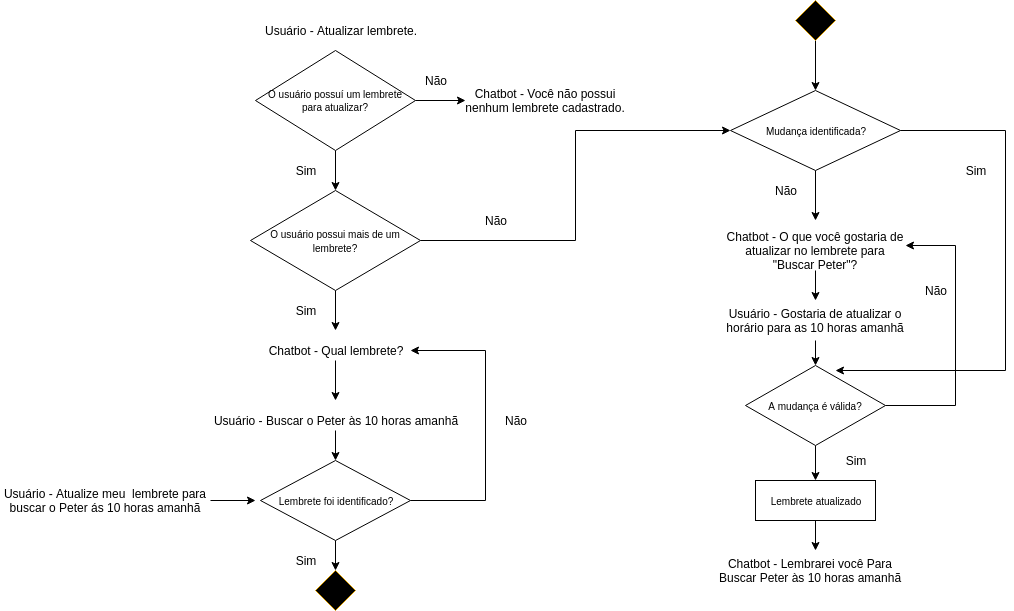
\includegraphics{imagens/Chatbot.png}
  \fonte{\cite{Samer}}
\end{figure}

Outra característica importante nesse tipo de \textit{chatbots}, é que eles não precisam necessariamente compreender a linguagem humana para executarem suas tarefas~\cite{Juliano}.

\section{\textit{Chatbots} de domínio amplo}\label{cap:02:sec:01:sub:02:bot-dominio}

Já os \textit{chatbots} de domínio amplo utilizam de recursos mais avançados de Inteligência Artificial (IA), são capazes de compreender o que o usuário solicita e podem relacionar-se a qualquer área de domínio de conhecimento~\cite{Juliano}. 
Na maior parte do tempo, o atendimento realizado por esse tipo de \textit{chatbots}, procura simular a conversação em linguagem humana.
Em outras palavras, um dos objetivos principais é responder perguntas de forma que os usuários tenham a impressão de estarem conversando com outra pessoa e não com um programa de computador.
Para isso, são utilizadas técnicas de Aprendizagem de Máquina (\textit{Machine Learning}) ou de Processamento de Linguagem Natural (\textit{Natural Language Processing})~\cite{Falaki}. 
Assim, o \textit{chatbot} é treinado com base nas interações dos usuários e consegue aprender com elas, se tornando mais inteligente e preciso ao decorrer deste processo.

As Assistentes Virtuais Inteligentes (AVIs) são um dos exemplos de \textit{chatbots} desse tipo. 
As AVIs são uma das principais tendências de soluções para otimizar o relacionamento entre empresas e consumidores~\cite{DDS}. 
Por meio de mecanismos de Inteligência Artificial, elas aprendem a partir das interações com o consumidor e, com isso, melhoram o seu repertório. 
Assim, são capazes de entender as necessidades do cliente e auxiliá-los da devida maneira na resolução de seus problemas.

\section{Inteligência artificial para \textit{chatbots}}\label{cap:02:sec:02:ia}

Nas subseções a seguir, serão detalhadas as duas técnicas mais utilizadas da IA para a criação de \textit{chatbots} de domínio amplo.

\subsection{Aprendizado de máquina}\label{cap:02:sec:02:sub:machine-learning}

De maneira simplificada, Aprendizagem de máquina é a prática de usar algoritmos para coletar dados, aprender com eles, e então fazer uma determinação ou predição sobre alguma atividade específica~\cite{MLSimple}. Assim ao invés de implementar as rotinas de software propriamente ditas, com um conjunto específico de instruções para completar uma tarefa em particular, a máquina é “treinada” usando uma quantidade grande de dados e algoritmos que dão e ela a habilidade de aprender como executar a tarefa. De maneira mais técnica, é um método de análise de dados que automatiza a construção de modelos analíticos~\cite{SASML}. Se baseia na ideia de que sistemas podem aprender com dados, identificar padrões e tomar decisões com o mínimo de intervenção humana.

Existem vários serviços que fornecem e facilitam o uso de tecnologias de aprendizagem de máquina, um deles, por exemplo, é a Amazon Machine Learning.
A Amazon Machine Learning oferece ferramentas e assistentes de visualização que orientam o desenvolvedor durante o processo de criação de modelos de aprendizado de máquina, sem necessidade de aprender tecnologias e algoritmos complexos para o desenvolvimento de tal. 


\subsection{Processamento de Linguagem Natural}\label{cap:02:sec:02:sub:pln}

O Processamento de Linguagem Natural (PLN) é a subárea da IA que estuda a capacidade e as limitações de uma máquina em entender a linguagem dos seres humanos~\cite{PLN1}.
Alguns dos objetivo do PLN é fornecer aos computadores a capacidade de  reconhecer o contexto, fazer análise sintática, semântica, léxica e morfológica, criar resumos, extrair informação, interpretar os sentidos, analisar sentimentos e até aprender conceitos com os textos processados~\cite{PLN1}.

Um dos métodos utilizados do PLN para o desenvolvimento de \textit{chatbots} é transformar uma sentença textual (dado) em informação (intenção e entidades)~\cite{Anatomy}. Em outras palavras, as intenções expressam funcionalidades, entidades expressam parâmetros para a execução de uma funcionalidade. Essas entidades precisam ser cadastradas, de forma a servir à base de conhecimento do PLN. Depois criamos as intenções, onde determinamos frases e sentenças que usarão essas entidades para expressar essas intenções. Assim, de modo simplório, o PLN passa a conseguir interpretar textos completos, textos simples e até mesmo incompletos.

Atualmente, existem vários serviços que dão suporte para a criação de PLN, um desses exemplos é o Wit.ia. Wit.ai é uma plataforma de desenvolvimento de PLN gratuita que transforma a linguagem natural (fala ou escrita) em dados estruturados. Um dos principais motivos para o uso do Wit.ai é por sua simplicidade no processo de criação de aplicativos e dispositivos com os quais as pessoas podem conversar, nesse contexto, na criação de \textit{chatbots}. Com isso, se abstrai a necessidade de aprender todo o processo de desenvolvimento de algoritmos de PLN.


\section{\textit{Chatbots} em plataformas de mensagens instantâneas}\label{cap:02:sec:03:sub:chatbotsmessenger}

Um mensageiro instantâneo consiste em um software que permite que diferentes usuários troquem mensagens, geralmente por escrito, em tempo real. 
Esses mensageiros instantâneos podem possuir alguns recursos adicionais como o envio de arquivos, conversas de áudio, conversas coletivas e até video conferências.
O termo mensageiro instantâneo, no entanto, encontra-se em desuso, sendo agora chamado com mais frequência por plataformas de mensagens instantâneas, ou simplesmente por \textit{messengers}. Podemos citar alguns \textit{messengers} como exemplo, tais como o Whatsapp, Telegram, WeChat, Slack, Facebook Messenger, entre outros.

No que se diz respeito à criação de \textit{chatbots}, alguns desses \textit{messengers} oferecem ferramentas e suporte, sob licenças especificas, para o desenvolvimento em sua plataforma, por meio de \textit{Application Programming Interfaces} (APIs).
Dentre os \textit{messengers}, um dos mais famosos por possuírem tais funcionalidades, é o Telegram.
O Telegram foi lançado em 2015 e possuí cerca de 100 milhões de usuários ativos mensais~\cite{IMaster}, 
É válido ressaltar também, os seus recursos avançados em questão de segurança e criptografia.
O Telegram oferece suporte para desenvolvimento de \textit{chatbots} desde 2015, por meio de sua API baseada no protocolo HTTP.


\section{Projetando \textit{chatbots}}\label{cap:02:sec:05:projeto}

Como sistemas computacionais são construídos para terem utilidade no mundo real, modelar o domínio de aplicação é uma atividade de suma importância.
A partir dessa atividade, pode se compreender a necessidade do sistema a ser construído e também definir os requisitos que tornam o sistema útil~\cite{ReqJair}. 
Pelo fato do \textit{chatbot} também se tratar de um produto digital, algumas práticas e estudos também devem ser realizados em seu processo de criação. Algumas dessas pŕaticas envolvem a análise e especificação dos requisitos e a elaboração dos diálogos que farão parte do repertório de um \textit{chatbot}.

\subsection{Análise e especificação dos requisitos}

De acordo com \alusao{ReqJair} a análise e especificação de requisitos de software envolve as atividades de determinar os objetivos de um software e as restrições associadas a ele.
\alusao{ReqJair} diz que a análise é o processo de observação e levantamento dos elementos do domínio no qual o sistema será introduzido. Deve-se identificar  as pessoas, atividades, informações do domínio para que se possa decidir o que deverá ser informatizado ou não.
Já a especificação é a descrição sistemática e abstrata do que o software deve fazer, a partir daquilo que foi analisado.

\subsubsection{Classificação de requisitos}\label{cap:02:sec:05:projeto:classificacao-requisitos}

\alusao{Sommerville} estabelece que os requisitos de um sistema são as descrições do que o sistema deve fazer, os serviços que oferece e as restrições a seu funcionamento.
Esses requisitos refletem as necessidades dos clientes para um sistema que serve a uma finalidade determinada, como controlar um dispositivo, efetuar um pedido ou encontrar informações.
É válido ressaltar que os requisitos de software são frequentemente classificados como requisitos funcionais e requisitos não funcionais.

Os requisitos funcionais de um sistema descrevem o que ele deve fazer.
Eles dependem do tipo de software a ser desenvolvido, de quem são seus possíveis usuários e da abordagem geral adotada pela organização ao escrever os requisitos~\cite{Sommerville}.
Quando expressos como requisitos de usuário, os requisitos funcionais são normalmente descritos de forma abstrata, para serem compreendidos pelos usuários do sistema.\label{texto:requisito_funcional}

Já os requisitos não funcionais, como o nome sugere, são requisitos que não estão diretamente relacionados com os serviços específicos oferecidos pelo sistema a seus usuários~\cite{Sommerville}.
Eles podem estar relacionados às propriedades emergentes do sistema, como confiabilidade, tempo de resposta, integridade, disponibilidade, ocupação de área entre outros.\label{texto:requisito_nao_funcional}

\subsection{Especificando requisitos utilizando casos de uso}

De acordo com \alusao{ReqJair} um caso de uso especifica o comportamento do sistema a ser desenvolvido sem, no entanto, especificar como este comportamento será implementado.
Os comportamentos descrevem as funções da aplicação que caracterizam a funcionalidade do sistema.
Um caso de uso representa o que o sistema faz e não como o sistema faz, proporcionando uma visão externa e não interna do sistema. Cada caso de uso define um requisito funcional do sistema~\cite{ReqJair}.

O caso de uso descreve um conjunto de sequências de ações que o sistema desempenha para produzir um resultado esperado pelo usuário.
Cada sequência representa a interação de entidades externas e o sistema~\cite{ReqJair}.
Estas entidades são chamadas de atores e que podem ser usuários ou outros sistemas.
No caso de usuários, um ator representa na verdade uma função de usuários. Para isso, normalmente se utiliza da notação \textit{Unified Modeling Language} (UML) como linguagem de especificação para representar os casos de uso. Na Figura~\ref{cap:02:fig:caso-de-uso-exemplo}, segue um exemplo de especificação de casos de uso utilizando a notação UML de um sistema de vendas.\label{texto:especificando-com-casos-de-uso}

\begin{figure}
  \caption{%
    \label{cap:02:fig:caso-de-uso-exemplo}
    Caso de uso - Sistema de Vendas
  }
  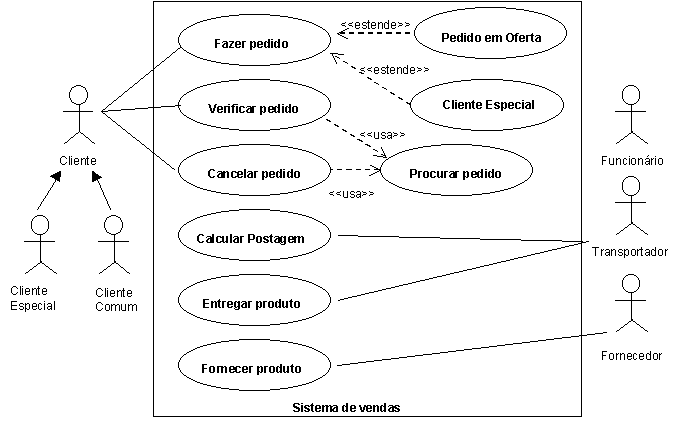
\includegraphics{imagens/casosd2.png}
  \fonte{\cite{ReqJair2}}
\end{figure}

\subsection{Elaboração dos diálogos de um \textit{chatbot} a partir de cenários}\label{texto:elaborando-dialogos}

Para a elaboração dos diálogos que irão fazer parte do repertório de um \textit{chatbot}, uma técnica utilizada para a sua modelagem e especificação se dá pelo uso dos cenários.
\alusao{ReqJair} diz que cenários consistem de uma coleção de narrativas de situações no domínio que favorecem o levantamento de informações, a identificação de problemas e a antecipação das soluções.
Cenários são uma maneira de representar, no contexto de \textit{chatbots}, os diálogos e interações e as possibilidades que podem surgir a partir destes. Abaixo, um exemplo de cenário que simula o diálogo entre uma atendente e um cliente que deseja consultar seu histórico de compras:


\subsection{Suposição inicial}
    
O cliente informa que deseja consultar o seu histórico de compras; a atendente pergunta suas informações pessoais (nome e CPF); o cliente informa seus dados; a atendente faz uma consulta com base nos dados adquiridos; a atendente exibe o histórico de compras do cliente.
    
\begin{enumerate}[label=\alph*)]
\tightlist
    \item \textbf{Cliente}: Gostaria de consultar meu histórico de compras, por favor.
   \item \textbf{Atendente}: O senhor poderia me informar o seu nome completo e os três últimos dígitos do seu CPF?
    \item \textbf{Cliente}: Claro. Meu nome é Custódio de Almeida, e os três últimos dígitos do meu CPF são 186.
    \item \textbf{Atendente}: Um instante, por favor.
    \item \textbf{Atendente}: O histórico do senhor é o seguinte: \\
    Dia: 20/02/2017 - 1 Tênis branco da marca X, 2 camisetas rosas da marca Y; Dia: 25/02/2017 - 2 shorts amarelos da marca Z.

\end{enumerate}
    
\subsection{O que pode dar errado}
    
As informações fornecidas pelo usuário não conferem com as cadastradas no banco de dados. A atendente informa o usuário que os dados informados não são válidos e pede para que ele tente novamente.
    
\begin{enumerate}[label=\alph*)]
\tightlist
    \item \textbf{Atendente}: Me desculpe, mas parece que os dados informados não conferem. Você poderia tentar novamente?
    \item \textbf{Cliente}: Certo. Tente os seguintes dados dessa vez\ldots
\end{enumerate}
    
O usuário nunca efetuou uma compra no estabelecimento. A atendente informa que o usuário não tem nenhuma compra na loja e informa as promoções disponíveis.
    
\begin{enumerate}[label=\alph*)]
\tightlist
    \item \textbf{Atendente}: Me desculpe, mas parece que o senhor não possui nenhuma compra em nossa loja.
    \item \textbf{Cliente}: Tudo bem, então.
    \item \textbf{Atendente}: Caso seja do seu interesse, nós estamos com uma promoção de 30\% de desconto na compra de qualquer camiseta da marca X. Você gostaria de dar uma olhada?
\end{enumerate}
    
\subsection{Estado do sistema na conclusão}
    
Após exibir o histórico do cliente, a atendente irá perguntar se o ele deseja mais alguma coisa.
    
\begin{enumerate}[label=\alph*)]
\tightlist
    \item \textbf{Atendente}: Esse é todo o seu histórico de compras em nossa loja. Existe mais alguma coisa em que eu possa lhe ajudar?
    \ldots
\end{enumerate}


\section{Desenvolvimento de \textit{chatbots}}\label{chatbot:dev}

No desenvolvimento de \textit{chatbots}, pode-se dizer que existem duas maneiras para a sua criação: utilizando ferramentas de plataformas de \textit{chatbots} ou não. Para melhor explicar a vantagens e desvantagens de cada modo, nas subseções abaixo, estes serão detalhados.

\subsection{Utilizando plataformas de \textit{chatbots}}\label{chatbot:dev:plat}

As plataformas de \textit{chatbots} são sistemas que oferecem serviços para facilitar a criação de \textit{chatbots} e sua integração com os  \textit{messengers}.
Basicamente, essas plataformas abstraem a necessidade de programar rotinas de códigos complexas, já oferecem recursos ou serviços de IA embutidos e também a tradução da aplicação, aonde o \textit{chatbot} poderá ser exportado e integrado para os mais diversos \textit{messengers}.
O intuito dessas plataformas, é elevar a produtividade dos desenvolvedores responsáveis pela criação do \textit{chatbot}.
Assim, ao facilitar o processo de criação, abstraindo várias etapas complexas e trabalhosas, eles serão capazes de desenvolverem o \textit{chatbot} em menos tempo.
Como exemplo dessas plataformas de \textit{chatbots}, podemos citar a Microsoft Bot Plataform, ChatScript, Pandorabots, Facebook Bots for Messenger, BLIP, entre outros.

Porém, para que possam se utilizar dos recursos mais avançados dessas plataformas, as empresas ou desenvolvedores contratantes devem efetuar os pagamentos, que podem variar de acordo com o tipo de serviço solicitado, podendo estes serviços serem mais caros de acordo com o número de usuários simultâneos que o \textit{chatbot} poderá atender, até, em questões de utilização de recursos mais sofisticados e personalizados para agilizar no desenvolvimento dos \textit{chatbots}. 


\subsection{Não utilizando plataformas de \textit{chatbots}}\label{chatbot:dev:nplat}

Caso o desenvolvedor opte pela não utilização dessas plataformas de \textit{chatbots}, ele poderá customizar a sua aplicação utilizando as tecnologias, ferramentas e serviços que lhe bem convir.
Por exemplo, ele poderá escolher desde de uma linguagem de programação específica, até qual serviço de IA (caso seja um \textit{chatbot} de domínio amplo) que ele irá utilizar no projeto.
Como dito na seção \ref{cap:02:sec:03:sub:chatbotsmessenger}, muitos \textit{messengers} oferecem suporte e serviços, por meio de suas APIs, que facilitam o processo de desenvolvimento e integração do \textit{chatbot} em sua plataforma.
Assim, o desenvolvedor poderá avaliar dentre os serviços oferecidos por esses \textit{messengers} e escolher qual lhe oferece mais benefícios.

É válido ressaltar a existência de bibliotecas e frameworks, criados por terceiros, que facilitam ainda mais no desenvolvimento de \textit{chatbots}, e também, na sua integração com algum \textit{messenger}.
Tanto as bibliotecas quanto os frameworks, oferecem uma interface mais simplificada, implementada em uma linguagem de programação específica, na qual possui um conjunto de classes, métodos e funções que o desenvolvedor poderá usufruir, afim de criar um \textit{chatbot} de maneira mais rápida.
Desde modo, etapas que tendem a ser mais repetitivas no processo de criação de \textit{chatbots}, como enviar ou receber requisições da API do \textit{messengers}, são abstraídas.

  % Capitulo 3: Terceiro capítulo (arquivo Includes/Capitulo3.tex)
  % MIT License
%
% Copyright (c) 2018 José Nascimento <joseaugustodearaujonascimento@gmail.com>
%
% Permission is hereby granted, free of charge, to any person obtaining a copy
% of this software and associated documentation files (the "Software"), to deal
% in the Software without restriction, including without limitation the rights
% to use, copy, modify, merge, publish, distribute, sublicense, and/or sell
% copies of the Software, and to permit persons to whom the Software is
% furnished to do so, subject to the following conditions:
%
% The above copyright notice and this permission notice shall be included in all
% copies or substantial portions of the Software.
%
% THE SOFTWARE IS PROVIDED "AS IS", WITHOUT WARRANTY OF ANY KIND, EXPRESS OR
% IMPLIED, INCLUDING BUT NOT LIMITED TO THE WARRANTIES OF MERCHANTABILITY,
% FITNESS FOR A PARTICULAR PURPOSE AND NONINFRINGEMENT. IN NO EVENT SHALL THE
% AUTHORS OR COPYRIGHT HOLDERS BE LIABLE FOR ANY CLAIM, DAMAGES OR OTHER
% LIABILITY, WHETHER IN AN ACTION OF CONTRACT, TORT OR OTHERWISE, ARISING FROM,
% OUT OF OR IN CONNECTION WITH THE SOFTWARE OR THE USE OR OTHER DEALINGS IN THE
% SOFTWARE.

\chapter{EV.G Virtual Assistant}

A EV.G Virtual Assistant (EVA) é um \textit{chatbot} de domínio amplo que será capaz de interagir com os alunos vinculados à EV.G na medida de suas necessidades.
Ela irá atender tais solicitações via mecanismo de conversação textual na plataforma de mensagens instantâneas chamada Telegram, no atendimento administrativo de uma secretaria acadêmica.

Por meio de EVA, os alunos vinculados à EV.G poderão usufruir de várias funcionalidades.
Eles irão gerenciar seus cursos visualizando o andamento das inscrições, 
terão acesso ao catálogo unificado, calendário de turmas, histórico escolar, 
e também, serão auxiliados no processo de emissão de certificado. 
Tudo por meio de um acesso único e simplificado.

\section{Requisitos de EVA}\label{especificacao-requisitos-eva}

Como dito \ref{cap:02:sec:05:projeto}, modelar o domínio de aplicação de um \textit{chatbot} é uma atividade importante, pois a partir desta, pode se compreender a necessidade do sistema a ser construído, e também, definir os requisitos que o tornam útil.
É interessante deixar claro, que todo o processo de levantamento e validação dos requisitos já foi realizado e entregue por parte da EV.G. 
Assim, não haverá nenhuma seção que aborde como se deu tal levantamento. 
Ao invés disso, os requisitos de EVA serão apenas detalhados nas subseções a seguir.

\subsection{Requisitos funcionais}

Na seção \ref{cap:02:sec:05:projeto:classificacao-requisitos}, foi explicado o que são os requisitos funcionais de um sistema. 
Abaixo, na Quadro \ref{Quadro:Quadro1}, estão listados os requisitos funcionais elencados para o sistema de EVA.

\begin{quadro}[htb!]
\caption{Detalhamento de requisitos funcionais de EVA}
% \textsf{\caption{Especificação de requisitos funcionais de EVA}}
\label{Quadro:Quadro1}
\begin{tabular}{|p{1.2cm}|p{3.5cm}|p{7.5cm}|}
  \hline
   \textbf{\#RF} & \textbf{Nome}  & \textbf{Descrição}  \\
    \hline
    RF01 & Conversação & Permitir que o usuário interaja com o \textit{chatbot} na língua portuguesa por meio de mensagens textuais em um \textit{messenger}. \\
    \hline
    RF02 & Compreensão & O \textit{chatbot} deve ser capaz de compreender o que o usuário solicita, através das mensagens textuais enviadas por ele, e tomar as devidas decisões para atende-lo. \\
    \hline
    RF03 & Autenticação & O \textit{chatbot} deve possuir uma forma de identificar o usuário que está solicitando acesso à aplicação. \\
   \hline
     RF04 & Visualizar o histórico escolar & O \textit{chatbot} deve informar ao usuário o seu histórico escolar completo caso seja solicitado por ele. \\
   \hline
    RF05 & Auxiliar na emissão de certificados & O \textit{chatbot} deve auxiliar o usuário no processo de emissão de certificados dos cursos concluídos por ele, caso seja solicitado por ele. \\
   \hline
    RF06 & Visualizar as inscrições de cursos em aberto & O \textit{chatbot} deve exibir ao usuário quais inscrições de cursos que estão abertas, caso seja solicitado por ele. \\
   \hline
\end{tabular}
\mfonte
\end{quadro}

\subsection{Requisitos não funcionais}\label{cap3-requisitos-nao-funcionais}

Na seção \ref{cap:02:sec:05:projeto:classificacao-requisitos}, foi explicado o que são os requisitos não funcionais de um sistema. 
Abaixo, na Quadro \ref{Quadro:Quadro2}, estão listados os requisitos não funcionais elencados para o sistema de EVA.

\begin{quadro}[htb!]
\caption{Detalhamento de requisitos não funcionais de EVA}
\label{Quadro:Quadro2}
\begin{tabular}{|p{1.2cm}|p{3.5cm}|p{7.5cm}|}
  \hline
   \textbf{\#RNF} & \textbf{Nome}  & \textbf{Descrição}  \\
   \hline
    RNF01 & Disponibilidade & O sistema deve estar disponível continuamente (24 horas / 7 dias por semana). \\
   \hline
    RNF02 & Confidencialidade (a) & O sistema deve garantir a visualização dos dados apenas pelo usuário associado. \\
   \hline
    RNF03 & Confidencialidade (b) & O sistema deve garantir que caso algum usuário falhe ao tentar se autenticar por três vezes consecutivas, bloqueie as tentativas de acesso dele durante 24 horas. \\
   \hline
   RNF04 & Portabilidade & O sistema deverá atender prioritariamente na plataforma de mensagens instantâneas Telegram. \\
   \hline
    RNF05 & Interoperabilidade & O sistema deverá se comunicar com algum serviço de Processamento de Linguagem Natural. \\
   \hline
    RNF06 & Implementação & O sistema deverá ser implementado utilizando a linguagem de programação Python. \\
   \hline
    RNF07 & Autenticação & A autenticação será pela confirmação de dados pessoais, neste caso pelo email e/ou CPF cadastrado. \\
   \hline
\end{tabular}
\mfonte
\end{quadro}\label{Quadro:3}

\section{Casos de uso de EVA}\label{casos-de-uso-eva}

Na seção \ref{texto:especificando-com-casos-de-uso}, foi descrito o que são casos de uso e como eles normalmente são utilizados durante o projeto de um sistema. 
Elaborar os casos de uso permite definir quais funções de aplicação que o sistema deverá oferecer ao usuário~\cite{ReqJair}. 
Para a sua especificação, serão utilizados também alguns dos requisitos funcionais e não funcionais, que foram detalhados na seção \ref{especificacao-requisitos-eva}, para que se possa descrever as funcionalidades do sistema com ainda mais propriedade. 
Nas subseções a seguir, será realizado todo o processo de especificação e detalhamento dos casos de uso de EVA.

\subsection{Especificação dos atores}

Um ator é algo com comportamento, tal como uma pessoa (identificada por seu papel), um sistema ou uma organização~\cite{CraigLarman}. 
No que se diz respeito a EVA, foram identificados como atores o Visitante e o Aluno. 
Ambos poderão interagir com EVA, por meio de mensagens textuais, porém com as devidas restrições. 
É válido ressaltar, que a EVA não entra como ator, já que será o próprio sistema na qual está sendo modelando. 
Na Quadro \ref{Quadro:Quadro3} os atores são especificados.

\begin{quadro}[htb!]
\caption{Especificação dos atores do sistema de EVA}
\label{Quadro:Quadro3}
\begin{tabular}{|p{2cm}|p{3cm}|p{7.5cm}|}
  \hline
   \textbf{\#ATOR} & \textbf{Nome}  & \textbf{Descrição}  \\
   \hline
    ATOR01 & Visitante & Qualquer pessoa que interaja com EVA sem estar devidamente autenticado e identificado no sistema. \\
   \hline
    ATOR02 & Aluno & Qualquer pessoa que interaja com EVA e esteja devidamente autenticado e identificado no sistema. \\
   \hline
\end{tabular}
\mfonte
\end{quadro}

\subsection{Especificação dos casos de uso}

Como dito no começo desta seção, casos de uso permitem definir as funções de aplicação que o sistema deverá oferecer para o usuário. A partir dos requisitos funcionais identificados para EVA, foram extraídos os casos de uso especificados na Quadro \ref{Quadro:Quadro4}.

\begin{quadro}[htb!]
\caption{Especificação dos casos de uso de EVA}
\label{Quadro:Quadro4}
\begin{tabular}{|p{2cm}|p{3cm}|p{7.5cm}|}
  \hline
   \textbf{\#UC} & \textbf{Nome}  & \textbf{Descrição}  \\
   \hline
    UC01 & Dialogar com EVA & Os usuários do sistema poderão dialogar com EVA por meio de mensagens textuais, na língua portuguesa, através de um \textit{messenger}. A partir dessa funcionalidade, o usuário irá acessar todas as demais.\\
   \hline
    UC02 & Efetuar login & Autenticação de um usuário, permitindo que ele tenha acesso às funcionalidades restritas de EVA. \\
   \hline
    UC03 & Visualizar histórico escolar completo & O usuário poderá solicitar a visualização do histórico de todos os cursos que ele esteve matriculado no âmbito da EV.G. \\
   \hline
    UC04 & Receber auxílio na emissão de certificados & O usuário poderá solicitar auxilio para a emissão dos certificados dos cursos no qual ele finalizou no âmbito da EV.G. \\
   \hline
    UC05 & Visualizar inscrições de cursos em aberto & O usuário poderá solicitar a visualização de todos os cursos na qual possui matricula ativa no âmbito da EV.G. \\
   \hline
    UC06 & Efetuar logout & O usuário deixará de estar autenticado no sistema. Com isso, ele volta a possuir acesso limitado às funcionalidades de EVA.\\
   \hline
\end{tabular}
\mfonte
\end{quadro}

\subsection{Diagrama de casos de uso}

Para descrever de forma visual e clara como se dará o vínculo entre os atores e os casos de uso identificados de EVA, foi criado um diagrama de casos de uso. Para a criação deste, foi utilizada a notação UML.

Na UML, os atores são representados como figuras ‘palito’. Cada caso de uso, que são as possíveis interações que poderão ser realizadas, é representada por uma elipse. As linhas fazem a ligação entre os atores e as interações. Na Figura \ref{cap:03:fig:diagrama}, está representado o diagrama de casos de uso de EVA.

\begin{figure}[htb!]
  \caption{
    \label{cap:03:fig:diagrama}
    Casos de uso - EVA
  }
  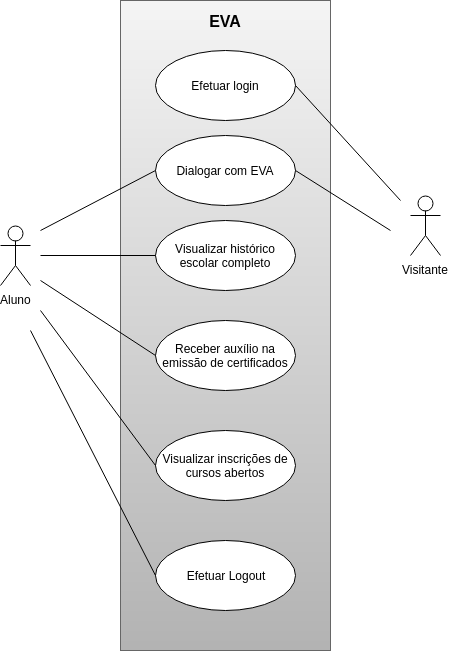
\includegraphics[width=0.3\linewidth]{imagens/CasoDeUsoEva.png}
  \mfonte
\end{figure}


\subsection{Detalhamento dos casos de uso}\label{cap3-detalhamento-casos-de-uso}

Nesta subseção, serão detalhados os casos de uso de EVA.

\subsubsection{UC01 - Dialogar com EVA}

\textbf{Descrição:} Este caso de uso especifica a ação principal de interação do usuário com o \textit{chatbot}, que é o diálogo. Por meio de mensagens textuais na língua portuguesa, o usuário poderá interagir com EVA e ter acesso à as suas funcionalidades. O nível de funcionalidades disponíveis para acesso do usuário, será determinada pelo fato dele estar autenticado ou não no sistema.

\subsubsubsection{Atores}
\begin{enumerate}[label=\alph*)]
    \tightlist
    \item ATOR01 - Visitante;
    \item ATOR02 - Aluno.
\end{enumerate}
        
\subsubsubsection{Requisitos funcionais}
\begin{enumerate}[label=\alph*)]
    \tightlist
        \item RF01 - Conversação;
        \item RF02 - Compreensão.
\end{enumerate}
        
\subsubsubsection{Requisitos não funcionais}
\begin{enumerate}[label=\alph*)]
    \tightlist
    \item RNF01 - Disponibilidade;
    \item RNF05 - Portabilidade;
    \item RNF05 - Interoperabilidade.
\end{enumerate}
        
\subsubsubsection{Fluxo básico}
\begin{enumerate}[label=\alph*)]
    \tightlist
    \item O usuário envia uma mensagem textual para EVA;
    \item EVA irá consultar sua base de conhecimento para compreender o que o ator solicita;
    \item EVA responde ao usuário com base no que foi compreendido.
\end{enumerate}

\subsubsection{UC02 - Efetuar login}

\textbf{Descrição:} Este caso de uso especifica a ação de autenticação no sistema, com o objetivo de identificar o aluno vinculado a EV.G. A partir da autenticação, O aluno passará a receber auxilio personalizado e terá acesso aos recursos mais sofisticados de EVA. O usuário irá informar o seu CPF ou e-mail, EVA irá consultar na sua base de dados afim de verificar se o usuário de fato possui um vinculo com a EV.G, e então será determinado se há a possibilidade de ser realizada a autenticação ou não.


\subsubsubsection{Atores}
\begin{enumerate}[label=\alph*)]
    \tightlist
    \item ATOR01 - Visitante;
    \item ATOR02 - Aluno.
\end{enumerate}
        
\subsubsubsection{Pré-condições}
\begin{enumerate}[label=\alph*)]
    \tightlist
    \item O usuário deve possuir um vinculo com a EV.G.
\end{enumerate}
        
\subsubsubsection{Pós-condições}
\begin{enumerate}[label=\alph*)]
    \tightlist
    \item O usuário terá acesso às funcionalidades mais personalizadas de EVA.
\end{enumerate}
        
\subsubsubsection{Requisitos funcionais}
        \begin{enumerate}[label=\alph*)]
        \tightlist
            \item RF01 - Conversação;
            \item RF02 - Compreensão;
            \item RF03 - Autenticação.
        \end{enumerate}
        
\subsubsubsection{Requisitos não funcionais}
\begin{enumerate}[label=\alph*)]
    \tightlist
    \item RNF01 - Disponibilidade;
    \item RNF02 - Confidencialidade (a);
    \item RNF03 - Confidencialidade (b);
    \item RNF05 - Interoperabilidade;
    \item RNF07 - Autenticação.
\end{enumerate}
        
\subsubsubsection{Fluxo básico}
    \begin{enumerate}[label=\alph*)]
    \tightlist
        \item Ao início de uma conversação com EVA, ela irá solicitar que o usuário se identifique, para que ela possa lhe dar auxilio mais personalizado. Para isso, EVA irá solicitar que ele lhe informe o seu CPF ou e-mail cadastrados na EV.G;
        \item O usuário então irá informar o seu e-mail ou CPF;
        \item EVA irá verificar se o usuário está bloqueado no sistema;
        \item EVA irá verificar se o número de tentativas de autenticação chegaram ao valor limite, nesse caso, a três;
        \item EVA irá consultar em sua base de dados se as informações de fato conferem;
        \item O sistema então irá autenticar o usuário;
        \item EVA dá as boas vindas e informa ao usuário que a autenticação foi efetuada com sucesso;
        \item EVA apresenta as suas funcionalidades ao usuário e o convida a utilizar alguma.
    \end{enumerate}
        
\subsubsubsection{Fluxo alternativo A}
        \begin{enumerate}[label=\alph*)]
        \tightlist
            \item No Passo \textit{e} do Fluxo Básico, após EVA consultar sua base de dados, foi visto que as informações não conferem;
            \item A contagem para o limite de tentativas de autenticação de um usuário é incrementada em um;
            \item EVA então informa ao usuário que os dados não conferem e pede para que ele informe o CPF ou o e-mail novamente;
            \item O fluxo retornar ao Passo \textit{b} do Fluxo básico.
        \end{enumerate}
        
\subsubsubsection{Fluxo alternativo B}
    \begin{enumerate}[label=\alph*)]
    \tightlist
        \item No Passo \textit{e} do Fluxo Básico, a mensagem textual enviada pelo usuário não aparenta ser nem algo parecido com CPF ou e-mail;
        \item EVA informa que ao usuário que ele precisa informar o CPF ou o e-mail para que ele possa se identificar, e assim, para que eles possam continuar dialogando;
        \item O fluxo retorna ao Passo \textit{b} do Fluxo básico.
    \end{enumerate}
        
\subsubsubsection{Fluxo alternativo C}
    \begin{enumerate}[label=\alph*)]
    \tightlist
        \item No Passo \textit{c} do Fluxo Básico, foi visto que o usuário está bloqueado no sistema;
        \item EVA informa que por questões de segurança, o usuário está bloqueado por um dia;
        \item EVA auxilia o usuário, que caso ele de fato ache que possui algum vinculo com a EV.G, que ele entre em contato através do e-mail da EVG;
        \item EVA informa o e-mail;
        \item EVA pede desculpa pelo transtorno.
    \end{enumerate}
        
\subsubsubsection{Fluxo alternativo D}
        \begin{enumerate}[label=\alph*)]
        \tightlist
            \item No Passo \textit{d} do Fluxo Básico, foi visto que o usuário tentou se autenticar por três vezes sem sucesso;
            \item EVA bloqueia o usuário por um dia;
            \item EVA informa que por questões de segurança, o usuário está bloqueado por um dia;
            \item EVA auxilia o usuário, que caso ele de fato ache que possui um vinculo com a EV.G, que ele entre em contato através do e-mail da EVG;
            \item EVA informa o e-mail;
            \item EVA pede desculpa pelo transtorno.
        \end{enumerate}

\subsubsection{UC03 - Visualizar histórico escolar completo}

\textbf{Descrição:} Este caso de uso especifica a funcionalidade de EVA de pesquisar e informar o histórico escolar de um aluno vinculado a EV.G. Para cada item identificado, EVA deve informar o nome do curso, a carga horária, o estado em que se encontra a inscrição do aluno e o estado de sua turma de ensino. 

\subsubsubsection{Atores}
    \begin{enumerate}[label=\alph*)]
        \tightlist
        \item ATOR02 - Aluno.
    \end{enumerate}
        
\subsubsubsection{Pré-condições}
    \begin{enumerate}[label=\alph*)]
        \tightlist
        \item O usuário deve estar autenticado no sistema.
    \end{enumerate}
        
\subsubsubsection{Requisitos funcionais}
    \begin{enumerate}[label=\alph*)]
        \tightlist
        \item RF01 - Conversação;
        \item RF02 - Compreensão;
        \item RF04 - Visualizar histórico escolar.
    \end{enumerate}
        
\subsubsubsection{Requisitos não funcionais}
    \begin{enumerate}[label=\alph*)]
        \tightlist
        \item RNF01 - Disponibilidade;
        \item RNF02 - Confidencialidade (a);
        \item RNF04 - Portabilidade;
        \item RNF05 - Interoperabilidade.
    \end{enumerate}
        
\subsubsubsection{Fluxo básico}
    \begin{enumerate}[label=\alph*)]
        \tightlist
        \item O aluno envia uma mensagem textual para EVA solicitando o seu histórico escolar;
        \item EVA irá consultar sua base de conhecimento para compreender o que o aluno solicita;
        \item EVA irá consultar a base de dados da EV.G para pesquisar os dados escolares do aluno;
        \item EVA irá formatar os dados encontrados para serem exibidos ao aluno;
        \item EVA irá informar ao aluno o seu histórico escolar completo. Para cada item identificado, EVA deverá especificar os nome do curso, a cargas horária, o estado da inscrição do aluno e o estado da turma de ensino;
    \end{enumerate}
        
\subsubsubsection{Fluxo alternativo A}
    \begin{enumerate}[label=\alph*)]
        \tightlist
        \item No Passo \textit{c} do Fluxo básico, foi constatado que o aluno não possui nenhuma matricula nos cursos da EV.G;
        \item EVA irá informar o aluno que ele não possui nenhuma matricula nos cursos da EV.G;
        \item EVA irá sugerir ao aluno que ele visite o site da EV.G para ter acesso ao catálogo dos cursos oferecidos pela instituição.
    \end{enumerate}


\subsubsection{UC04 - Receber auxílio na emissão de certificados}

\textbf{Descrição:} Este caso de uso especifica a funcionalidade de EVA de auxiliar o aluno vinculado a EV.G no processo de emissão de certificado. EVA irá pesquisar os cursos concluídos pelo aluno, e a partir destes, irá informar-lo quais procedimentos ele deverá realizar para emitir o certificado. Existem três situações possíveis para a emissão de certificados. O primeira situação, caso o curso tenha sido concluído no ano de 2015 para frente, EVA deve orientar o aluno a emitir o certificado no ambiente https://ava.enap.gov.br. O segundo, caso o curso tenha sido concluído entre os anos de 2013 a 2014, EVA deve orientar o aluno a emitir o certificado no ambiente https://moodle23.enap.gov.br. E o último, caso o curso tenha sido concluído antes do ano de 2013, EVA deverá orientar o aluno a enviar um e-mail para ead@enap.gov.br. Além das instruções para a emissão do certificado, para os itens de cada caso, EVA deverá informar o nome do curso e a carga horária.

\subsubsubsection{Atores}
    \begin{enumerate}[label=\alph*)]
        \tightlist
        \item ATOR02 - Aluno.
    \end{enumerate}
        
\subsubsubsection{Pré-condições}
    \begin{enumerate}[label=\alph*)]
        \tightlist
        \item O usuário deve estar autenticado no sistema.
    \end{enumerate}
        
\subsubsubsection{Requisitos funcionais}
    \begin{enumerate}[label=\alph*)]
        \tightlist
        \item RF01 - Conversação;
        \item RF02 - Compreensão;
        \item RF05 - Auxiliar na emissão de certificados.
    \end{enumerate}
        
\subsubsubsection{Requisitos não funcionais}
    \begin{enumerate}[label=\alph*)]
        \tightlist
        \item RNF01 - Disponibilidade;
        \item RNF02 - Confidencialidade (a);
        \item RNF04 - Portabilidade;
        \item RNF05 - Interoperabilidade.
    \end{enumerate}
        
\subsubsubsection{Fluxo básico}
    \begin{enumerate}[label=\alph*)]
        \tightlist
        \item O aluno envia uma mensagem textual para EVA solicitando ajuda na emissão dos certificados;
        \item EVA irá consultar sua base de conhecimento para compreender o que o aluno solicita;
        \item EVA irá consultar a base de dados da EV.G para pesquisar os dados escolares do aluno;
        \item EVA irá formatar os dados encontrados para serem exibidos ao aluno;
        \item EVA irá auxiliar o aluno, com base no ano de conclusão dos cursos encontrados, quais procedimentos ele deverá realizar. Para cada situação, EVA informará o nome do curso e a carga horária de cada item.
    \end{enumerate}
        
\subsubsubsection{Fluxo alternativo A}
    \begin{enumerate}[label=\alph*)]
        \tightlist
        \item No Passo \textit{c}  do Fluxo principal, foi constatado que o aluno não concluiu nenhum curso da EV.G;
        \item EVA irá informar oa aluno que ele não concluiu nenhum curso da EV.G, logo, não tem como auxiliá-lo na emissão de certificados;
        \item EVA irá sugerir o aluno que ele visite o site da EV.G para ter acesso ao catálogo dos cursos oferecidos pela instituição.
    \end{enumerate}


\subsubsection{UC05 - Visualizar inscrições de cursos em aberto}
\textbf{Descrição:} Este caso de uso especifica a funcionalidade de EVA de pesquisar e informar quais inscrições de cursos de um aluno vinculado a EV.G que estão em aberto. Para cada item identificado, EVA deve informar o nome do curso, a carga horária, estado da matricula do aluno e o estado da turma. 

\subsubsubsection{Atores}
    \begin{enumerate}[label=\alph*)]
        \tightlist
        \item ATOR02 - Aluno.
    \end{enumerate}
        
\subsubsubsection{Pré-condições}

    \begin{enumerate}[label=\alph*)]
        \tightlist
        \item O usuário deve estar autenticado no sistema.
    \end{enumerate}
        
\subsubsubsection{Requisitos funcionais}
    \begin{enumerate}[label=\alph*)]
        \tightlist
        \item RF01 - Conversação;
        \item RF02 - Compreensão;
        \item RF06 - Visualizar as inscrições de cursos em aberto.
    \end{enumerate}
        
\subsubsubsection{Requisitos não funcionais}
    \begin{enumerate}[label=\alph*)]
        \tightlist
        \item RNF01 - Disponibilidade;
        \item RNF02 - Confidencialidade (a);
        \item RNF04 - Portabilidade;
        \item RNF05 - Interoperabilidade.
    \end{enumerate}
        
\subsubsubsection{Fluxo básico}
    \begin{enumerate}[label=\alph*)]
        \tightlist
        \item O aluno envia uma mensagem textual para EVA solicitando que deseja saber quais cursos que estão em aberto;
        \item EVA irá consultar sua base de conhecimento para compreender o que o aluno solicita;
        \item EVA irá consultar a base de dados da EV.G para pesquisar os dados escolares do aluno;
        \item EVA irá formatar os dados encontrados para serem exibidos ao aluno;
        \item EVA irá informar ao aluno quais cursos que estão em aberto. Para cada item identificado, EVA deverá especificar o nome do curso, o estado da inscrição, a carga horária e a situação da turma. 
    \end{enumerate}
        
\subsubsubsection{Fluxo alternativo A}
    \begin{enumerate}[label=\alph*)]
        \tightlist
        \item No Passo \textit{c} do Fluxo básico, foi constatado que o aluno não possui inscrição em nenhum curso da EV.G;
        \item EVA irá informar ao aluno que ele não possui nenhuma inscrição nos cursos da EV.G;
        \item EVA irá sugerir o aluno que ele visite o site da EV.G para ter acesso ao catálogo dos cursos oferecidos pela instituição.
    \end{enumerate}

    
\subsubsection{UC06 - Efetuar logout}

\textbf{Descrição:} Este caso de uso especifica a funcionalidade onde o usuário deixará de estar autenticado no sistema.

\subsubsubsection{Atores}
    \begin{enumerate}[label=\alph*)]
        \tightlist
        \item ATOR01 - Visitante;
        \item ATOR02 - Aluno.
    \end{enumerate}
        
\subsubsubsection{Pré-condições}
    \begin{enumerate}[label=\alph*)]
        \tightlist
        \item O usuário deve estar autenticado no sistema.
    \end{enumerate}
        
\subsubsubsection{Pós-condições}
    \begin{enumerate}[label=\alph*)]
        \tightlist
        \item O usuário deixará de estar autenticado no sistema, voltando a ter acesso limitado às funcionalidades de EVA.
    \end{enumerate}
        
\subsubsubsection{Requisitos funcionais}
    \begin{enumerate}[label=\alph*)]
        \tightlist
        \item RF01 - Conversação;
        \item RF02 - Compreensão.
    \end{enumerate}
        
\subsubsubsection{Requisitos não funcionais}
        \begin{enumerate}[label=\alph*)]
        \tightlist
            \item RNF01 - Disponibilidade;
            \item RNF02 - Confidencialidade (a);
            \item RNF04 - Portabilidade;
            \item RNF05 - Interoperabilidade.
        \end{enumerate}
        
\subsubsubsection{Fluxo básico}
    \begin{enumerate}[label=\alph*)]
        \tightlist
        \item O aluno envia uma mensagem textual para EVA solicitando que deseja efetuar o logout;
        \item EVA irá consultar sua base de conhecimento para compreender o que o aluno solicita;
        \item EVA irá desvincular o aluno de sua base de conhecimento;
        \item O aluno passa a ser um visitante;            \item EVA irá informar de que o logout foi feito com sucesso.
    \end{enumerate}


\section{Modelagem dos diálogos de EVA}

Na seção \ref{texto:elaborando-dialogos} foi explicado como elaborar diálogos de um \textit{chatbot} a partir de cenários. Já na seção \ref{casos-de-uso-eva}, foram especificados e detalhados os casos de uso de EVA. Nesta seção, serão elaborados os diálogos, com base nos casos de uso de EVA, utilizando os cenários de cada um deles. É válido ressaltar, que existirão variações nas mensagens enviadas por EVA como resposta nos cenários especificados, porém, essas mensagens serão posteriormente cadastradas pela administração da EV.G.

\subsection{Cenários}

Nesta subseção, serão detalhados os diálogos de EVA utilizando os cenários.

\subsubsection{Diálogo UC01 - Dialogar com EVA}

Especificação do cenário relacionado ao UC01 - Dialogar com EVA.

\subsubsubsection{Suposição inicial}
    
    O usuário envia uma mensagem textual para EVA; EVA consulta sua base de conhecimento para compreender o que o ator solicita; EVA responde ao usuário.
    
    \begin{enumerate}[label=\alph*)]
        \tightlist
        \item \textbf{Usuário:} Olá, quem é você?
        \item \textbf{EVA:} Eu sou a EVA, a sua secretaria virtual da EVG. Eu posso pesquisar o seu histórico escolar, te auxiliar na emissão de certificados e também informar quais cursos estão em aberto!! Como posso lhe ser útil?
    \end{enumerate}
    
\subsubsubsection{O que pode dar errado}
    
O usuário não autenticado solicitar o uso de alguma funcionalidade restrita de EVA.
    
    \begin{enumerate}[label=\alph*)]
        \tightlist
            \item \textbf{Usuário:} Informe o meu histórico escolar.
            \item \textbf{EVA:} Você ainda não está autenticado no nosso sistema. Por favor, se identifique me enviando seu e-mail ou CPF.
        \end{enumerate}
    
O usuário solicitar algo que EVA não compreende.
    
    \begin{enumerate}[label=\alph*)]
        \tightlist
        \item \textbf{Usuário:} EVA, existe vida após a morte?
        \item \textbf{EVA:} Nossa, mil perdões, mas realmente eu não consegui entender o que você precisa.
    \end{enumerate}

\subsubsection{Diálogo UC02 - Efetuar login}

Especificação do cenário relacionado ao UC02 - Efetuar login.

\subsubsubsection{Suposição inicial} 
    
EVA solicita que o usuário se identifique para que ela possa lhe dar auxilio mais personalizado; EVA solicita que o usuário informe o seu CPF ou o e-mail; o usuário informa o seu CPF ou e-mail; EVA informa que estará consultando as credenciais em seu banco de dados; EVA dá as boas vindas ao aluno.
        
\begin{enumerate}[label=\alph*)]
        \tightlist
    \item \textbf{EVA:} Você ainda não está cadastrado no nosso sistema. Por favor, se identifique me enviando seu e-mail ou CPF.
    \item \textbf{Usuário:} test@evg.com.
    \item \textbf{EVA:} Certo.. Aguarde alguns instantes enquanto eu faço a consulta no nosso banco de dados, está bem?
    \item \textbf{EVA:} Seja muito bem-vindo!! Eu sou a EVA, a sua assistente virtual da EV.G. Eu posso pesquisar o seu histórico escolar, te auxiliar na emissão de certificados e também informar a você quais cursos estão em aberto!! Fique a vontade, faça alguma pergunta.
\end{enumerate}
    
\subsubsubsection{O que pode dar errado}
    
As credenciais informadas pelo usuário não conferem.
        
\begin{enumerate}[label=\alph*)]
        \tightlist
    \item \textbf{EVA:} Ops!! Parece que os dados informados não conferem. Por favor, tente novamente.
\end{enumerate}
        
O usuário envia uma mensagem textual que não é nada parecido com CPF ou e-mail.

\begin{enumerate}[label=\alph*)]
        \tightlist
    \item \textbf{EVA:} Por favor, informe o seu e-mail ou o seu CPF. Caso você não tenha essas informações cadastradas, peço que entre em contato com a EV.G.
\end{enumerate}
        
O usuário tentou se autenticar por três vezes consecutivas sem sucesso.

\begin{enumerate}[label=\alph*)]
        \tightlist
    \item \textbf{EVA:} Infelizmente, por motivos de segurança, estaremos bloqueando suas solicitações de registro por um dia. Caso você ache que os dados inseridos estão corretos, peço que você entre em contato com a EV.G. Tente novamente amanhã, desculpe o transtorno.
\end{enumerate}
        
O usuário, já bloqueado, tenta se autenticar novamente.

\begin{enumerate}[label=\alph*)]
        \tightlist
    \item \textbf{EVA:} Por motivos de segurança, você está bloqueado por um dia. Caso você ache que os dados inseridos anteriormente estejam corretos, peço que você entre em contato com a EV.G. Tente novamente amanhã, desculpe o transtorno.
\end{enumerate}

\subsubsection{Diálogo UC03 - Visualizar histórico escolar completo}

Especificação do cenário relacionado ao UC03 - Visualizar histórico escolar completo.

\subsubsubsection{Suposição inicial}
    
O aluno envia uma mensagem textual para EVA solicitando o seu histórico escolar; EVA irá consultar a base de dados da EV.G para pesquisar os dados do histórico do aluno; EVA se desculpa por ter deixado o aluno esperando; EVA informa o histórico escolar do aluno.
        
\begin{enumerate}[label=\alph*)]
        \tightlist
    \item \textbf{Aluno:} EVA, gostaria de verificar meu histórico escolar, por favor.
    \item \textbf{EVA:} Só um segundo.
    \item \textbf{EVA:} Desculpe a demora! Aqui estão os dados que você solicitou.
    \item \textbf{EVA:} Curso: Informática básica; Carga horária: 70 horas; Situação da inscrição: Concluído;
    Situação da turma: Finalizada.
\end{enumerate}
    
\subsubsubsection{O que pode dar errado}
    
O usuário não possui nenhuma inscrição nos cursos da EV.G.
        
\begin{enumerate}[label=\alph*)]
        \tightlist
    \item \textbf{EVA:} Parece que você não tem nenhuma informação a ser exibida.
    \item \textbf{EVA:} Porque você não inicia um curso na nossa plataforma? Para ter acesso ao catálogo dos cursos da EV.G, acesse: https://evg.gov.br/catalogo.
\end{enumerate}
    
\subsubsubsection{Estado do sistema na conclusão}
    
Após atender o aluno, EVA irá perguntar se o mesmo deseja mais alguma coisa.
        
\begin{enumerate}[label=\alph*)]
        \tightlist
    \item \textbf{EVA:} Deseja mais alguma coisa?
\end{enumerate}

\subsubsection{Diálogo UC04 - Receber auxílio na emissão de certificados}

Especificação do cenário relacionado ao UC04 - Receber auxílio na emissão de certificados.

\subsubsubsection{Suposição inicial}
    
O aluno envia uma mensagem textual para EVA solicitando auxilio na emissão de certificados; EVA irá consultar a base de dados da EV.G para pesquisar os dados dos cursos concluídos do aluno; EVA se desculpa por ter deixado o aluno esperando; EVA auxilia o aluno no processo de emissão de certificado.
        
\begin{enumerate}[label=\alph*)]
        \tightlist
            \item \textbf{Aluno:} Eu gostaria de auxílio na emissão dos meus certificados, por favor.
            \item \textbf{EVA:} Só um segundo.
            \item \textbf{EVA:} Desculpe a demora! Aqui estão os dados que você solicitou.
            \item \textbf{EVA:} Você finalizou o(s) seguinte(s) curso(s) no período de 2015 em diante: Empreendedorismo (CH - 50 horas) e Gestão de negócios (CH - 60 horas). \\
            Para emitir o certificado de algum curso relacionado acima, acesse: https://ava.enap.gov.br.
            \item \textbf{EVA:} Você finalizou o(s) seguinte(s) curso(s) no período de 2013 a 2014: Introdução a vigilância sanitária (CH - 60 horas). \\
            Para emitir o certificado de algum curso relacionado acima, acesse: https://moodle23.enap.gov.br/.
            \item \textbf{EVA:} Você finalizou o(s) seguinte(s) curso(s) no período anterior a 2013: Federalismo fiscal no Brasil (CH - 50 horas). \\
            Para emitir o certificado de algum curso relacionado acima, envie um e-mail para 'ead@enap.gov.br', com o título do curso que você deseja emitir o certificado, o seu nome e CPF.
\end{enumerate}
    
\subsubsubsection{O que pode dar errado}
    
O usuário não possui nenhuma inscrição nos cursos da EV.G.
        
\begin{enumerate}[label=\alph*)]
        \tightlist
    \item \textbf{EVA:} Parece que você não tem nenhuma informação a ser exibida.
    \item \textbf{EVA:} Porque você não inicia um curso na nossa plataforma? Para ter acesso ao catálogo dos cursos da EV.G, acesse: https://evg.gov.br/catalogo.
\end{enumerate}
    
\subsubsubsection{Estado do sistema na conclusão}
    
Após atender o aluno, EVA irá perguntar se o mesmo deseja mais alguma coisa.
        
\begin{enumerate}[label=\alph*)]
        \tightlist
    \item \textbf{EVA:} Deseja mais alguma coisa?
\end{enumerate}


\subsubsection{Diálogo UC05 - Visualizar inscrições de cursos em aberto}

Especificação do cenário relacionado ao UC05 - Visualizar inscrições de cursos em aberto.

\subsubsubsection{Suposição inicial:}
    
O aluno envia uma mensagem textual para EVA solicitando a visualização dos cursos em aberto; EVA irá consultar a base de dados da EV.G para pesquisar os dados dos cursos que estão em aberto do aluno; EVA se desculpa por ter deixado o aluno esperando; EVA informa o aluno quais são os seus cursos em aberto.
        
\begin{enumerate}[label=\alph*)]
        \tightlist
    \item \textbf{Aluno:} Gostaria de ver os cursos que estão em andamento.
    \item \textbf{EVA:} Só um segundo.
    \item \textbf{EVA:} Desculpe a demora! Aqui estão os dados que você solicitou
    \item \textbf{EVA:} Curso: Ética e Serviço público; Carga horária: 20 horas; Situação da inscrição: Em andamento; Situação da turma: Aberto.
\end{enumerate}
    
\subsubsubsection{O que pode dar errado}
    
O usuário não possui nenhuma inscrição nos cursos da EV.G.
    
\begin{enumerate}[label=\alph*)]
        \tightlist
    \item \textbf{EVA:} Parece que você não tem nenhuma informação a ser exibida.
    \item \textbf{EVA:} Porque você não inicia um curso na nossa plataforma? Para ter acesso ao catálogo dos cursos da EV.G, acesse: https://evg.gov.br/catalogo.
\end{enumerate}
    
\subsubsubsection{Estado do sistema na conclusão}
    
Após atender o aluno, EVA irá perguntar se o mesmo deseja mais alguma coisa.
        
\begin{enumerate}[label=\alph*)]
        \tightlist
        \item \textbf{EVA:} Deseja mais alguma coisa?
\end{enumerate}

\subsubsection{Diálogo UC06 - Efetuar logout}

Especificação do cenário relacionado ao UC06 - Efetuar logout.

\subsubsubsection{Suposição inicial}
    
O aluno envia uma mensagem textual para EVA solicitando que deseja efetuar o logout no sistema.
        
\begin{enumerate}[label=\alph*)]
        \tightlist
    \item \textbf{Aluno:} EVA, gostaria de efetuar o logout.
    \item \textbf{EVA:} Só um segundo.
    \item \textbf{EVA:} O logout foi efetuado com sucesso. Lembre-se, sempre que desejar eu estarei por aqui, basta apenas informar o seu e-mail ou CPF. Até logo!
\end{enumerate}
    
\subsubsubsection{Estado do sistema na conclusão:}
    
O aluno deixa de estar autenticado no sistema de EVA.


\section{Arquitetura de EVA}

Na seção ~\ref{chatbot:dev}, foram exemplificadas as duas formas utilizadas no desenvolvimento de \textit{chatbots}, que são utilizando plataformas de \textit{chatbots} ou não. Para o desenvolvimento de EVA, foi optado pela não utilização dessas plataformas. Assim, será necessário que haja uma explicação a cerca das tecnologias utilizadas, e também, da arquitetura escolhida para a sua criação.

No que diz respeito a arquitetura de EVA, pode-se dizer que esta consiste em duas partes principais: a API e o \textit{chatbot} propriamente dito. A escolha desta divisão, está diretamente ligada ao fato de que o sistema, no futuro, tende a continuar crescendo, seja atendendo em outras plataformas de mensagens ou adicionando novas funcionalidades ao sistema de EVA. Em outras palavras, essa arquitetura tem como objetivo tornar o sistema mais escalável. Nas subseções abaixo, serão detalhados as tecnologias que irão compor todo o sistema de EVA e também detalhes sobre a sua implementação.

\subsection{Tecnologias}

Nesta subseção, serão detalhadas as principais tecnologias utilizadas em todo o desenvolvimento de EVA, tanto para a criação da API, quanto para o \textit{chatbot} propriamente dito.

\subsubsection{Python}

A linguagem de programação base de todo o sistema de EVA, é o Python. Numa breve descrição sobre a linguagem, pode-se citar que ela é multi paradigma, suportando o paradigma orientado a objetos, imperativo, funcional e procedural; possui também tipagem dinâmica, onde não se é necessário declarações dos tipos de dados que serão utilizados durante a programação; e também, por possuir diversos frameworks e bibliotecas que facilitam no desenvolvimento de aplicações.

A escolha do Python como linguagem base para o desenvolvimento de EVA, se deu a partir da experiência do autor com a mesma, e também, pela liberdade de escolha por parte da EV.G.

\subsubsection{Wit.ai}

Por se tratar de um \textit{chatbot} de domínio amplo, o sistema de EVA necessariamente precisa utilizar de algum recurso de IA, como abordado na seção \ref{cap:02:sec:01:sub:02:bot-dominio}. Para isso, pode-se utilizar técnicas de Aprendizagem de Máquina, descrita na seção \ref{cap:02:sec:02:sub:machine-learning} ou de PLN, descrita na seção \ref{cap:02:sec:02:sub:pln}.

Para o desenvolvimento de EVA, fará-se uso da técnica de PLN. Porém, para se abstrair da necessidade de aprender todo o processo de desenvolvimento de algoritmos de PLN, serão utilizados os serviços oferecidos pelo Wit.ai.

 Wit.ai é uma plataforma de desenvolvimento de PLN gratuita que transforma a linguagem natural (fala ou escrita) em dados estruturados (intenções). É válido ressaltar também, que o Wit.ai oferece uma biblioteca para a utilização dos seus serviços em Python, sendo este, um dos principais motivos para a sua escolha.

\subsubsection{Django}

Django é um framework gratuito e de código aberto para a criação de aplicações web, escrito em Python. Por ser um framework web, Django possui um conjunto de componentes que ajudam a desenvolver aplicações web de maneira simples e rápida.

Ele será utilizado para criar a API de EVA, na qual esta terá duas principais funções no sistema como um todo. A primeira, será armazenar a base de dados dos alunos da EV.G, para que se possa consultar as informações escolares dos alunos que estiverem se comunicando com o \textit{chatbot}. A segunda, é que a API estará responsável também por estabelecer uma interoperabilidade com o serviço de PNL fornecido pelo Wit.ai, para que possa compreender a mensagem textual enviada pelo usuário, e atende-lo de maneira eficiente.

\subsubsection{Python-telegram-bot}

Como EVA irá atender as solicitações dos alunos vinculados a EV.G pelo Telegram, será necessário que haja uma forma de integração do \textit{chatbot} com este \textit{messenger}. Atualmente, o Telegram possui o Telegram Bot API, que é uma API baseada no protocolo HTTP, criada para que desenvolvedores interessados possam construir \textit{chatbots} em sua plataforma.

Como o Python é a linguagem de programação base do sistema de EVA, e para facilitar ainda mais a integração do sistema com o Telegram Bot API, foi utilizado a biblioteca Python-telegram-bot. Esta biblioteca fornece uma interface de fácil acesso, em Python, aos recursos fornecidos pelo Telegram Bot API, se tornando uma solução ideal para a construção do sistema de EVA.

\subsection{Arquitetura da API}\label{eva-arquitetura-api}

Como dito no começo desta seção, o sistema de EVA é divido em duas partes principais, a API e o \textit{chatbots} propriamente dito. Nesta subseção, será explicado como funcionará a API de EVA.

O acrônimo API que provém do inglês Application Programming Interface (Em português, significa Interface de Programação de Aplicações), trata-se de um conjunto de rotinas e padrões estabelecidos e documentados por uma aplicação, para que outras aplicações consigam utilizar as funcionalidades desta, sem precisar conhecer detalhes da implementação do software. Desta forma, as APIs permitem uma interoperabilidade entre aplicações.

A API de EVA será desenvolvida utilizando o framework Django, e terá duas principais funções no sistema como um todo. A primeira, será que a API estará responsável por estabelecer uma interoperabilidade com o serviço de PNL fornecido pelo Wit.ai, para que possa compreender as mensagens textuais enviadas pelos alunos que estiverem se comunicando com o \textit{chatbot} de EVA. A segunda, será que a partir da intenção da mensagem, analisada e estruturada pelo Wit.ai, será elaborada a devida resposta e enviada de volta ao \textit{chatbot} de EVA.

É válido informar também, que a base de dados das informações escolares dos alunos vinculados a EV.G, estará atrelada à própria API de EVA, sendo assim, não será necessário que haja uma comunicação com algum serviço externo da EV.G, para que se possa consultar tais informações.

Para melhor exemplificar como funcionará a API de EVA, na Figura \ref{cap:03:fig:diagrama-sequencia-1} está apresentado o diagrama de sequência da mesma.

\begin{figure}
  \caption{
    \label{cap:03:fig:diagrama-sequencia-1}
    Diagrama de sequência da API de EVA
  }
  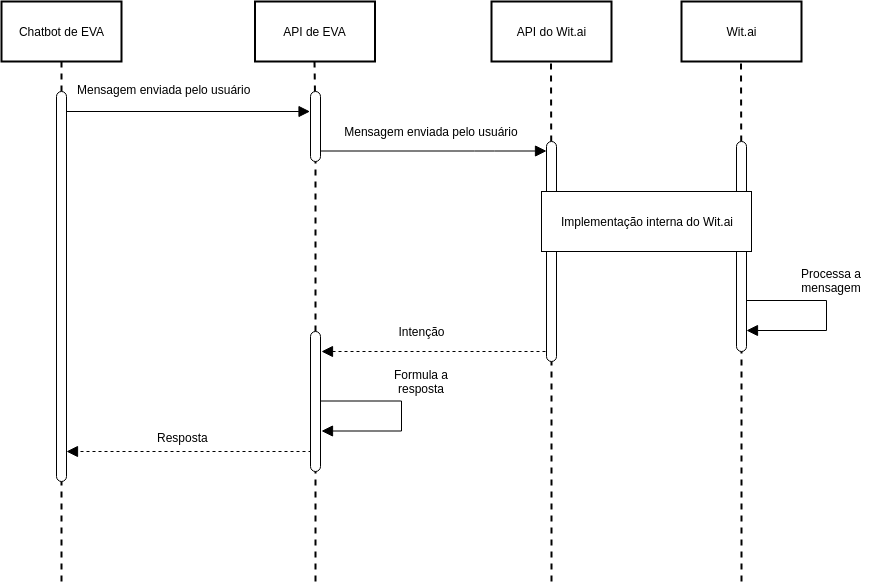
\includegraphics[width=0.7\linewidth]{imagens/EVAAPISEQUENCE.png}
  \mfonte
\end{figure}

\subsection{Arquitetura do \textit{chatbot}}\label{eva-arquitetura-chatbot}

Nesta subseção, será explicado como funcionará o \textit{chatbot} de EVA. Na seção \ref{cap:02:sec:03:sub:chatbotsmessenger}, foi detalhado como funcionam os \textit{chatbots} em plataformas de mensagens instantâneas. Lá foi explicado que alguns desses \textit{messengers} oferecem ferramentas e suporte, sob licenças específicas, para o desenvolvimento de \textit{chatbots} em sua plataforma, por meio de APIs. Como é um requisito essencial que EVA atenda as demandas dos usuários através do Telegram, será necessário que haja uma comunicação entre o sistema de EVA com a API do mesmo. Atualmente, o Telegram possui o Telegram Bot API, que é uma API baseada no protocolo HTTP, criada para que desenvolvedores interessados possam construir \textit{chatbots} em sua plataforma.

Para facilitar, em termos de desenvolvimento, a criação do \textit{chatbot} e integração com a Telegram Bot API, foi utilizado a biblioteca Python-telegram-bot. Esta biblioteca oferece uma interface, em Python, de fácil acesso aos recursos oferecidos pelo Telegram Bot API.

Na implementação do código do \textit{chatbot} de EVA, utilizando a biblioteca Python-telegram-bot, foi desenvolvido uma sub-rotina, que confere constantemente se há novas mensagens enviadas por algum usuário no \textit{messenger}. Caso haja, esta mensagem será enviada para a API de EVA para que possa ser compreendida e tratada de maneira devida. Quando a resposta for retornada, esta será formatada, para que então, possa ser enviada ao usuário no Telegram.

Resumidamente, esta parte do sistema de EVA será responsável por verificar se há novas mensagens enviada pelos usuários, estabelecer uma interoperabilidade com a API de EVA para que se possa analisar, compreender e atender as mensagens que foram enviadas pelos usuários, e por fim, formatar e enviar a mensagem de resposta ao usuário no Telegram. Para melhor detalhar o fluxo de interações, na Figura \ref{cap:03:fig:diagrama-sequencia-2} é apresentado o diagrama de sequência do \textit{chatbot} de EVA.

\begin{figure}
  \caption{
    \label{cap:03:fig:diagrama-sequencia-2}
    Diagrama de sequência do \textit{chatbot} de EVA
  }
  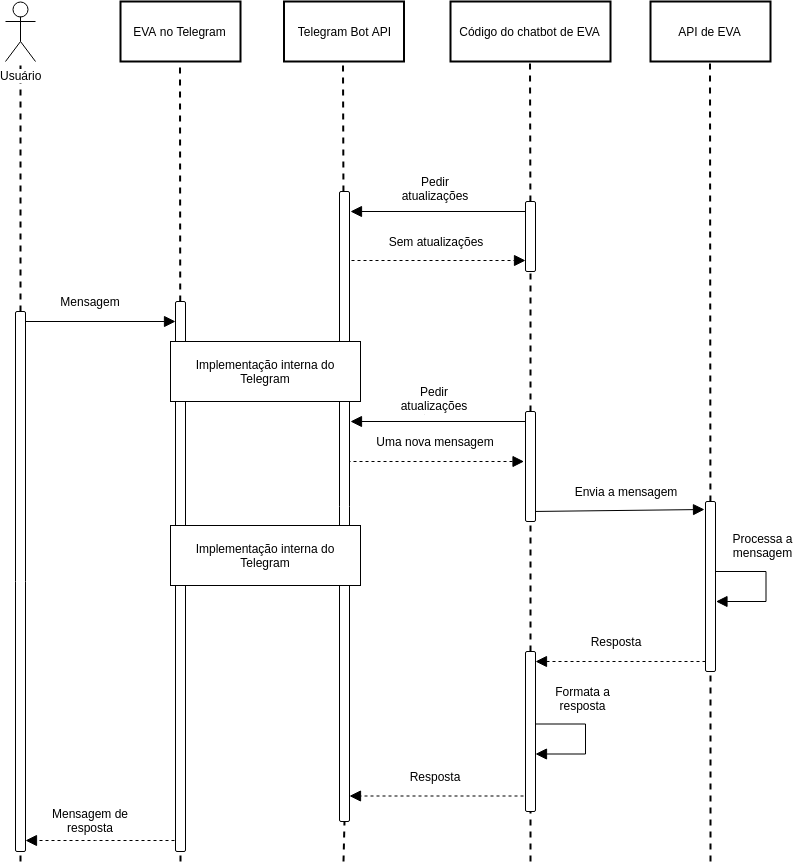
\includegraphics[width=0.5\linewidth]{imagens/EVACHATBOTSEQUENCE.png}
  \mfonte
\end{figure}

\subsection{Fluxo de comunicação das arquiteturas de EVA}

Para melhor exemplificar como se dá o fluxo de comunicação, processamento e resposta de EVA, desde a mensagem enviada pelo usuário até a sua resposta de EVA para o mesmo, na Figura \ref{cap:03:fig:processamento} é apresentada de maneira mais visual de como ocorre a comunicação entre as arquiteturas e os serviços utilizados no projeto.

\begin{figure}
  \caption{
    \label{cap:03:fig:processamento}
    Fluxo de comunicação de EVA
  }
  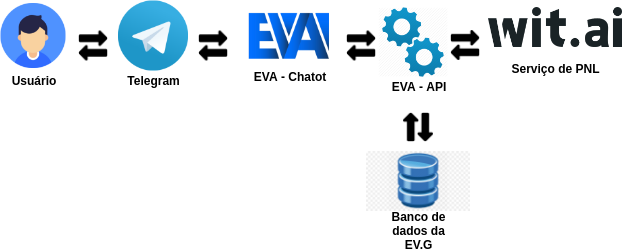
\includegraphics[width=0.8\linewidth]{imagens/EVADiagramComplete.png}
  \mfonte
\end{figure}

%--

  % Capitulo 4: Quarto capítulo (arquivo Includes/Capitulo4.tex)
  % MIT License
%
% Copyright (c) 2018 José Nascimento <joseaugustodearaujonascimento@gmail.com>
%
% Permission is hereby granted, free of charge, to any person obtaining a copy
% of this software and associated documentation files (the "Software"), to deal
% in the Software without restriction, including without limitation the rights
% to use, copy, modify, merge, publish, distribute, sublicense, and/or sell
% copies of the Software, and to permit persons to whom the Software is
% furnished to do so, subject to the following conditions:
%
% The above copyright notice and this permission notice shall be included in all
% copies or substantial portions of the Software.
%
% THE SOFTWARE IS PROVIDED "AS IS", WITHOUT WARRANTY OF ANY KIND, EXPRESS OR
% IMPLIED, INCLUDING BUT NOT LIMITED TO THE WARRANTIES OF MERCHANTABILITY,
% FITNESS FOR A PARTICULAR PURPOSE AND NONINFRINGEMENT. IN NO EVENT SHALL THE
% AUTHORS OR COPYRIGHT HOLDERS BE LIABLE FOR ANY CLAIM, DAMAGES OR OTHER
% LIABILITY, WHETHER IN AN ACTION OF CONTRACT, TORT OR OTHERWISE, ARISING FROM,
% OUT OF OR IN CONNECTION WITH THE SOFTWARE OR THE USE OR OTHER DEALINGS IN THE
% SOFTWARE.

\chapter{Simulação da interação de um aluno com EVA}

Por meio de simulações de interações com os alunos da EV.G, neste capítulo, serão apresentadas as principais funcionalidades desenvolvidas de EVA, que estará vinculada à plataforma de mensagens instantâneas Telegram. É válido salientar, que por motivos de segurança e integridade, como estão sendo utilizados dados reais dos alunos vinculados a EV.G, em algumas figuras foram postas tarjas pretas sob informações que são consideradas pessoais do usuário.

\section{Preparando o ambiente para as simulações}

Antes de iniciar de fato as simulações, necessita-se que o sistema de EVA esteja em execução.
Como este trabalho tende a ficar desatualizado, seja por questões tecnológicas ou até dado a alguma mudança no escopo do projeto por parte da EV.G, as instruções para configurar e instalar todas as dependências do sistema estarão disponíveis, e também, estarão sendo atualizadas com frequência no repositório oficial do projeto, que pode ser acessado pelo endereço eletrônico "http://github.com/evatalk".

\section{Iniciando uma conversa}

Como EVA está vinculada ao Telegram, inicialmente necessitará a instalação e execução deste \textit{messenger} em algum aparelho de telefone celular. Tendo isto em mente, basta acessar a opção "pesquisar" no Telegram, digitar "@evgvirtualassistantbot" e clicar na primeira opção de resposta. Logo em seguida, ao inicializar uma conversa com EVA, ela dará as boas-vindas e irá solicitar ao usuário que o mesmo se autentique, fornecendo o CPF ou o e-mail cadastrado na EV.G. Na Figura \ref{cap:04:fig:apresentacao-boas-vindas} é demonstrada tal situação.

\begin{figure}
  \caption{
    \label{cap:04:fig:apresentacao-boas-vindas}
    EVA - Boas-vindas
  }
  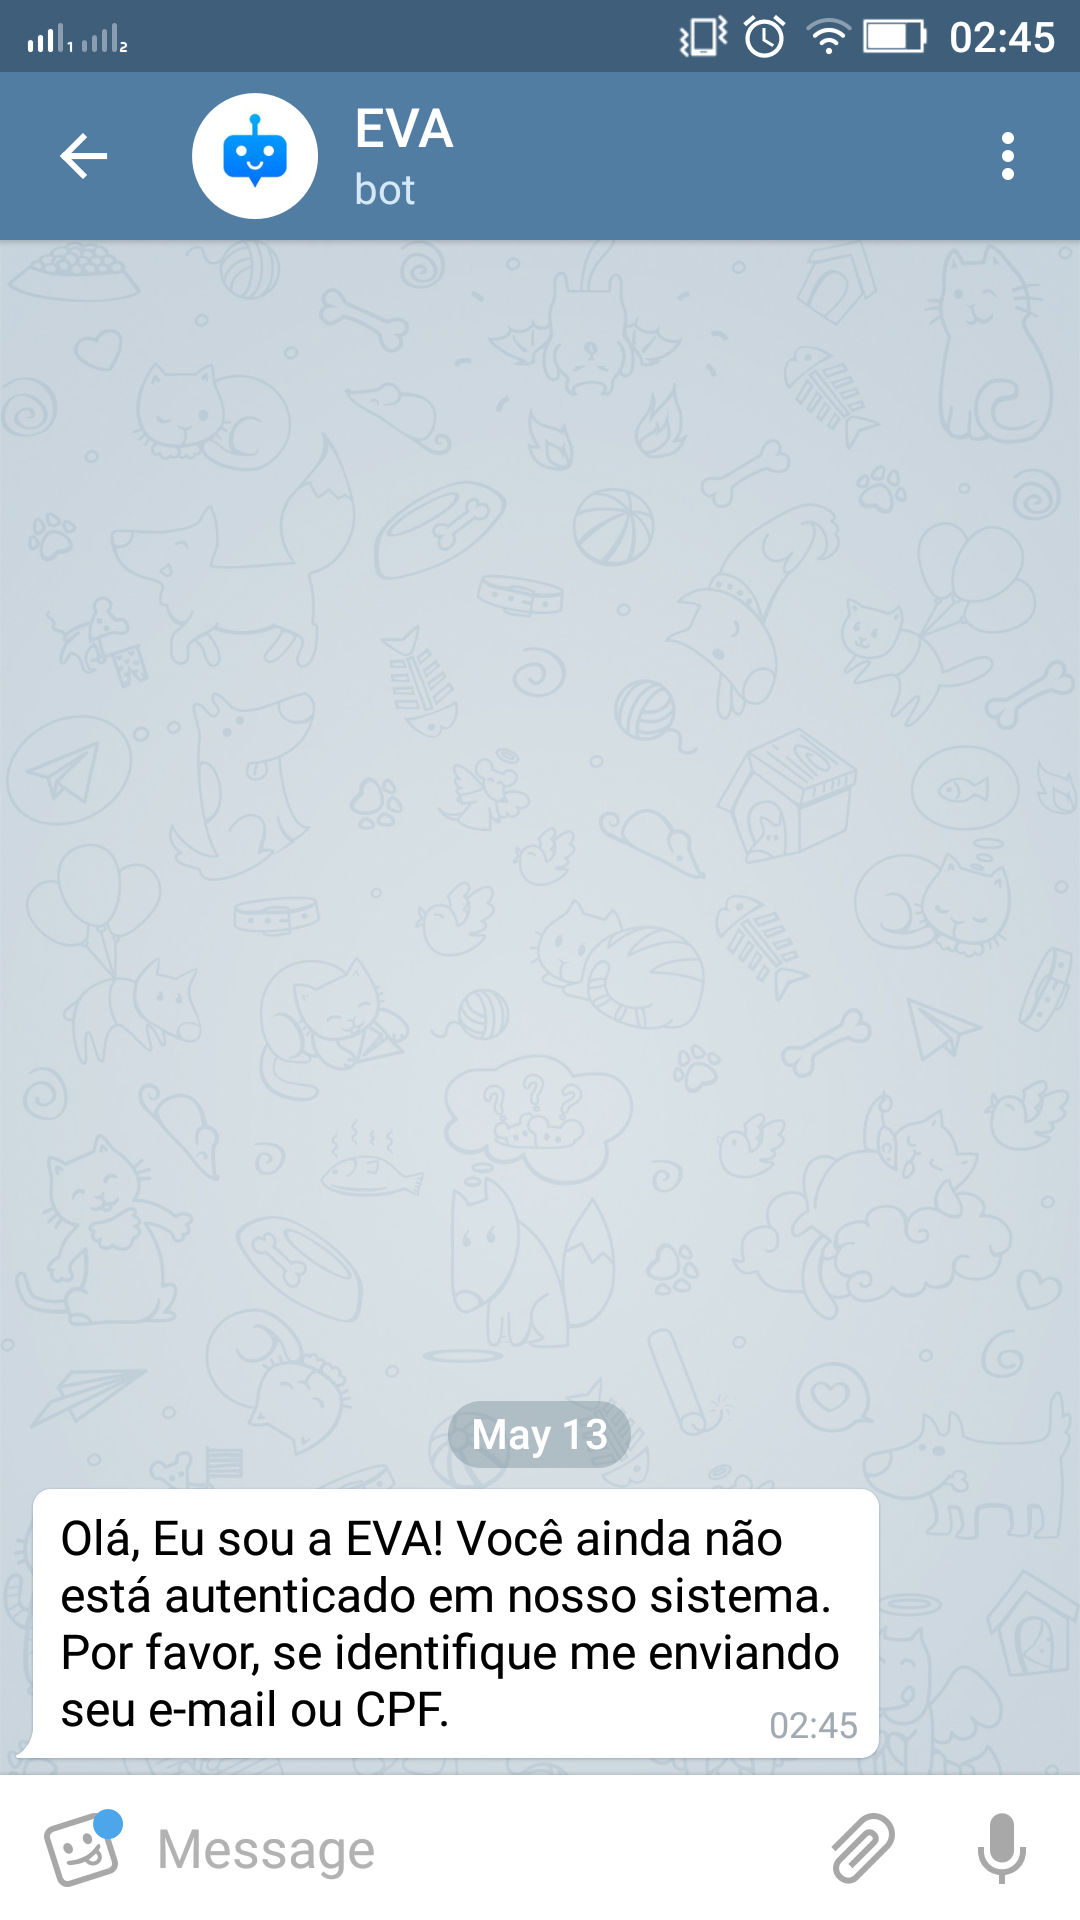
\includegraphics[width=0.2\linewidth]{imagens/apresentacao-boas-vindas.png}
  \mfonte
\end{figure}

\section{Autenticando}
O usuário poderá se autenticar para usufruir das funcionalidades mais sofisticadas de EVA. Para essa funcionalidade existem dois cenários possíveis: O de falha e o de sucesso na autenticação.

\subsection{Falha na autenticação}
Caso as credenciais fornecidas pelo usuário não estiverem corretas, EVA irá enviar uma mensagem dizendo que os dados não conferem e irá solicitar que o usuário informe o CPF ou o e-mail novamente. Se o usuário tentar se autenticar sem sucesso por três vezes consecutivas, o sistema irá bloqueá-lo por 24 horas e o \textit{chatbot} irá informar tal acontecimento ao usuário. Essas situações são apresentadas na Figura \ref{cap:04:fig:apresentacao-autenticação-falha}.

\begin{figure}
  \caption{
    \label{cap:04:fig:apresentacao-autenticação-falha}
    EVA - Bloqueio de usuário
  }
  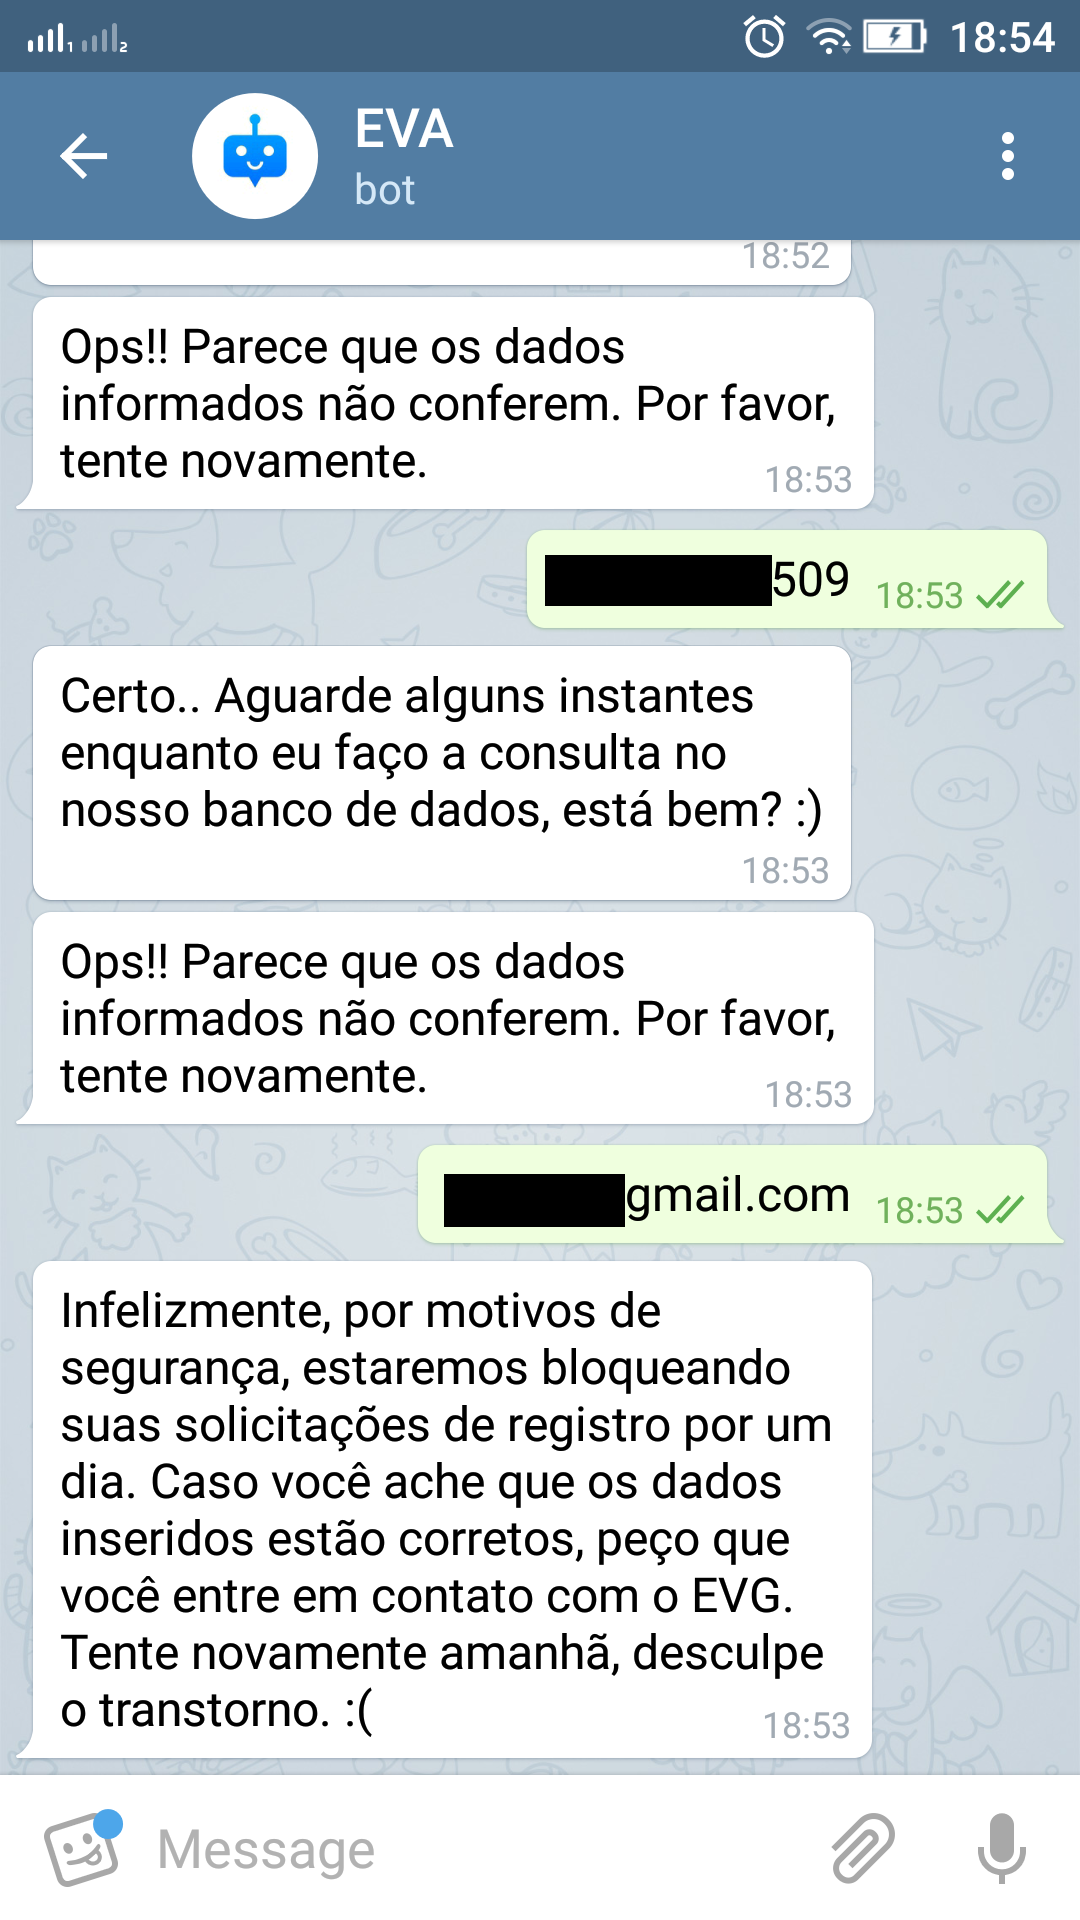
\includegraphics[width=0.2\linewidth]{imagens/apresentacao-autenticacao-falha.png}
  \mfonte
\end{figure}

\subsection{Sucesso na autenticação}
O aluno conseguiu se autenticar com sucesso no sistema e passará a ter acesso às funcionalidades mais sofisticadas de EVA. Na Figura \ref{cap:04:fig:apresentacao-autenticação-sucesso} este caso é apresentado.

\begin{figure}
  \caption{
    \label{cap:04:fig:apresentacao-autenticação-sucesso}
    EVA - Autenticação realizada com sucesso
  }
  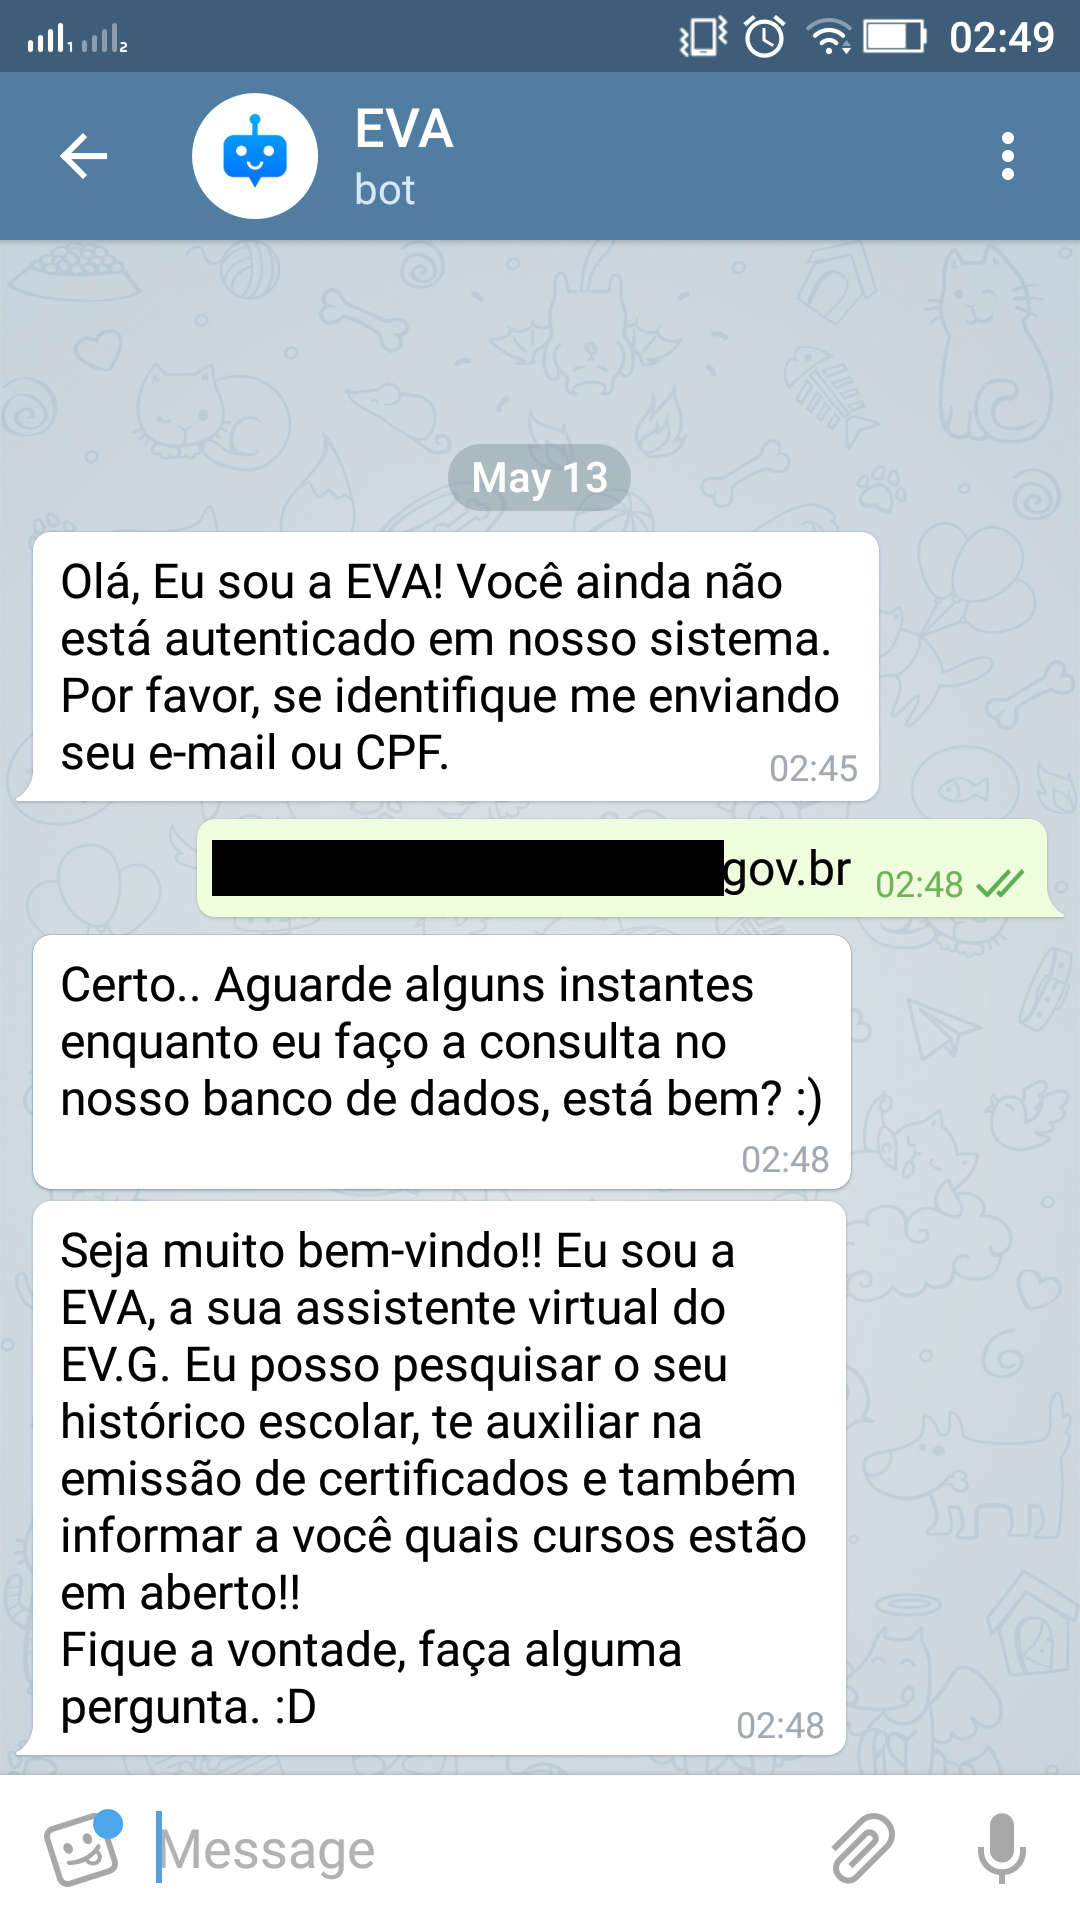
\includegraphics[width=0.2\linewidth]{imagens/apresentacao-autenticacao-sucesso.png}
  \mfonte
\end{figure}

\section{Dialogando com EVA}

Por se tratar de um \textit{chatbot} de domínio amplo, EVA compreende algumas nuances nas mensagens enviadas por um aluno, compreendendo quais funcionalidades ele deseja utilizar e também sabendo quando um usuário está a cumprimentando, xingando e até mesmo quando recebe mensagens de afeto, como mostrada na Figura \ref{cap:04:fig:apresentacao-dialogos}.

\begin{figure}
  \caption{
    \label{cap:04:fig:apresentacao-dialogos}
    EVA - Dialogando
  }
  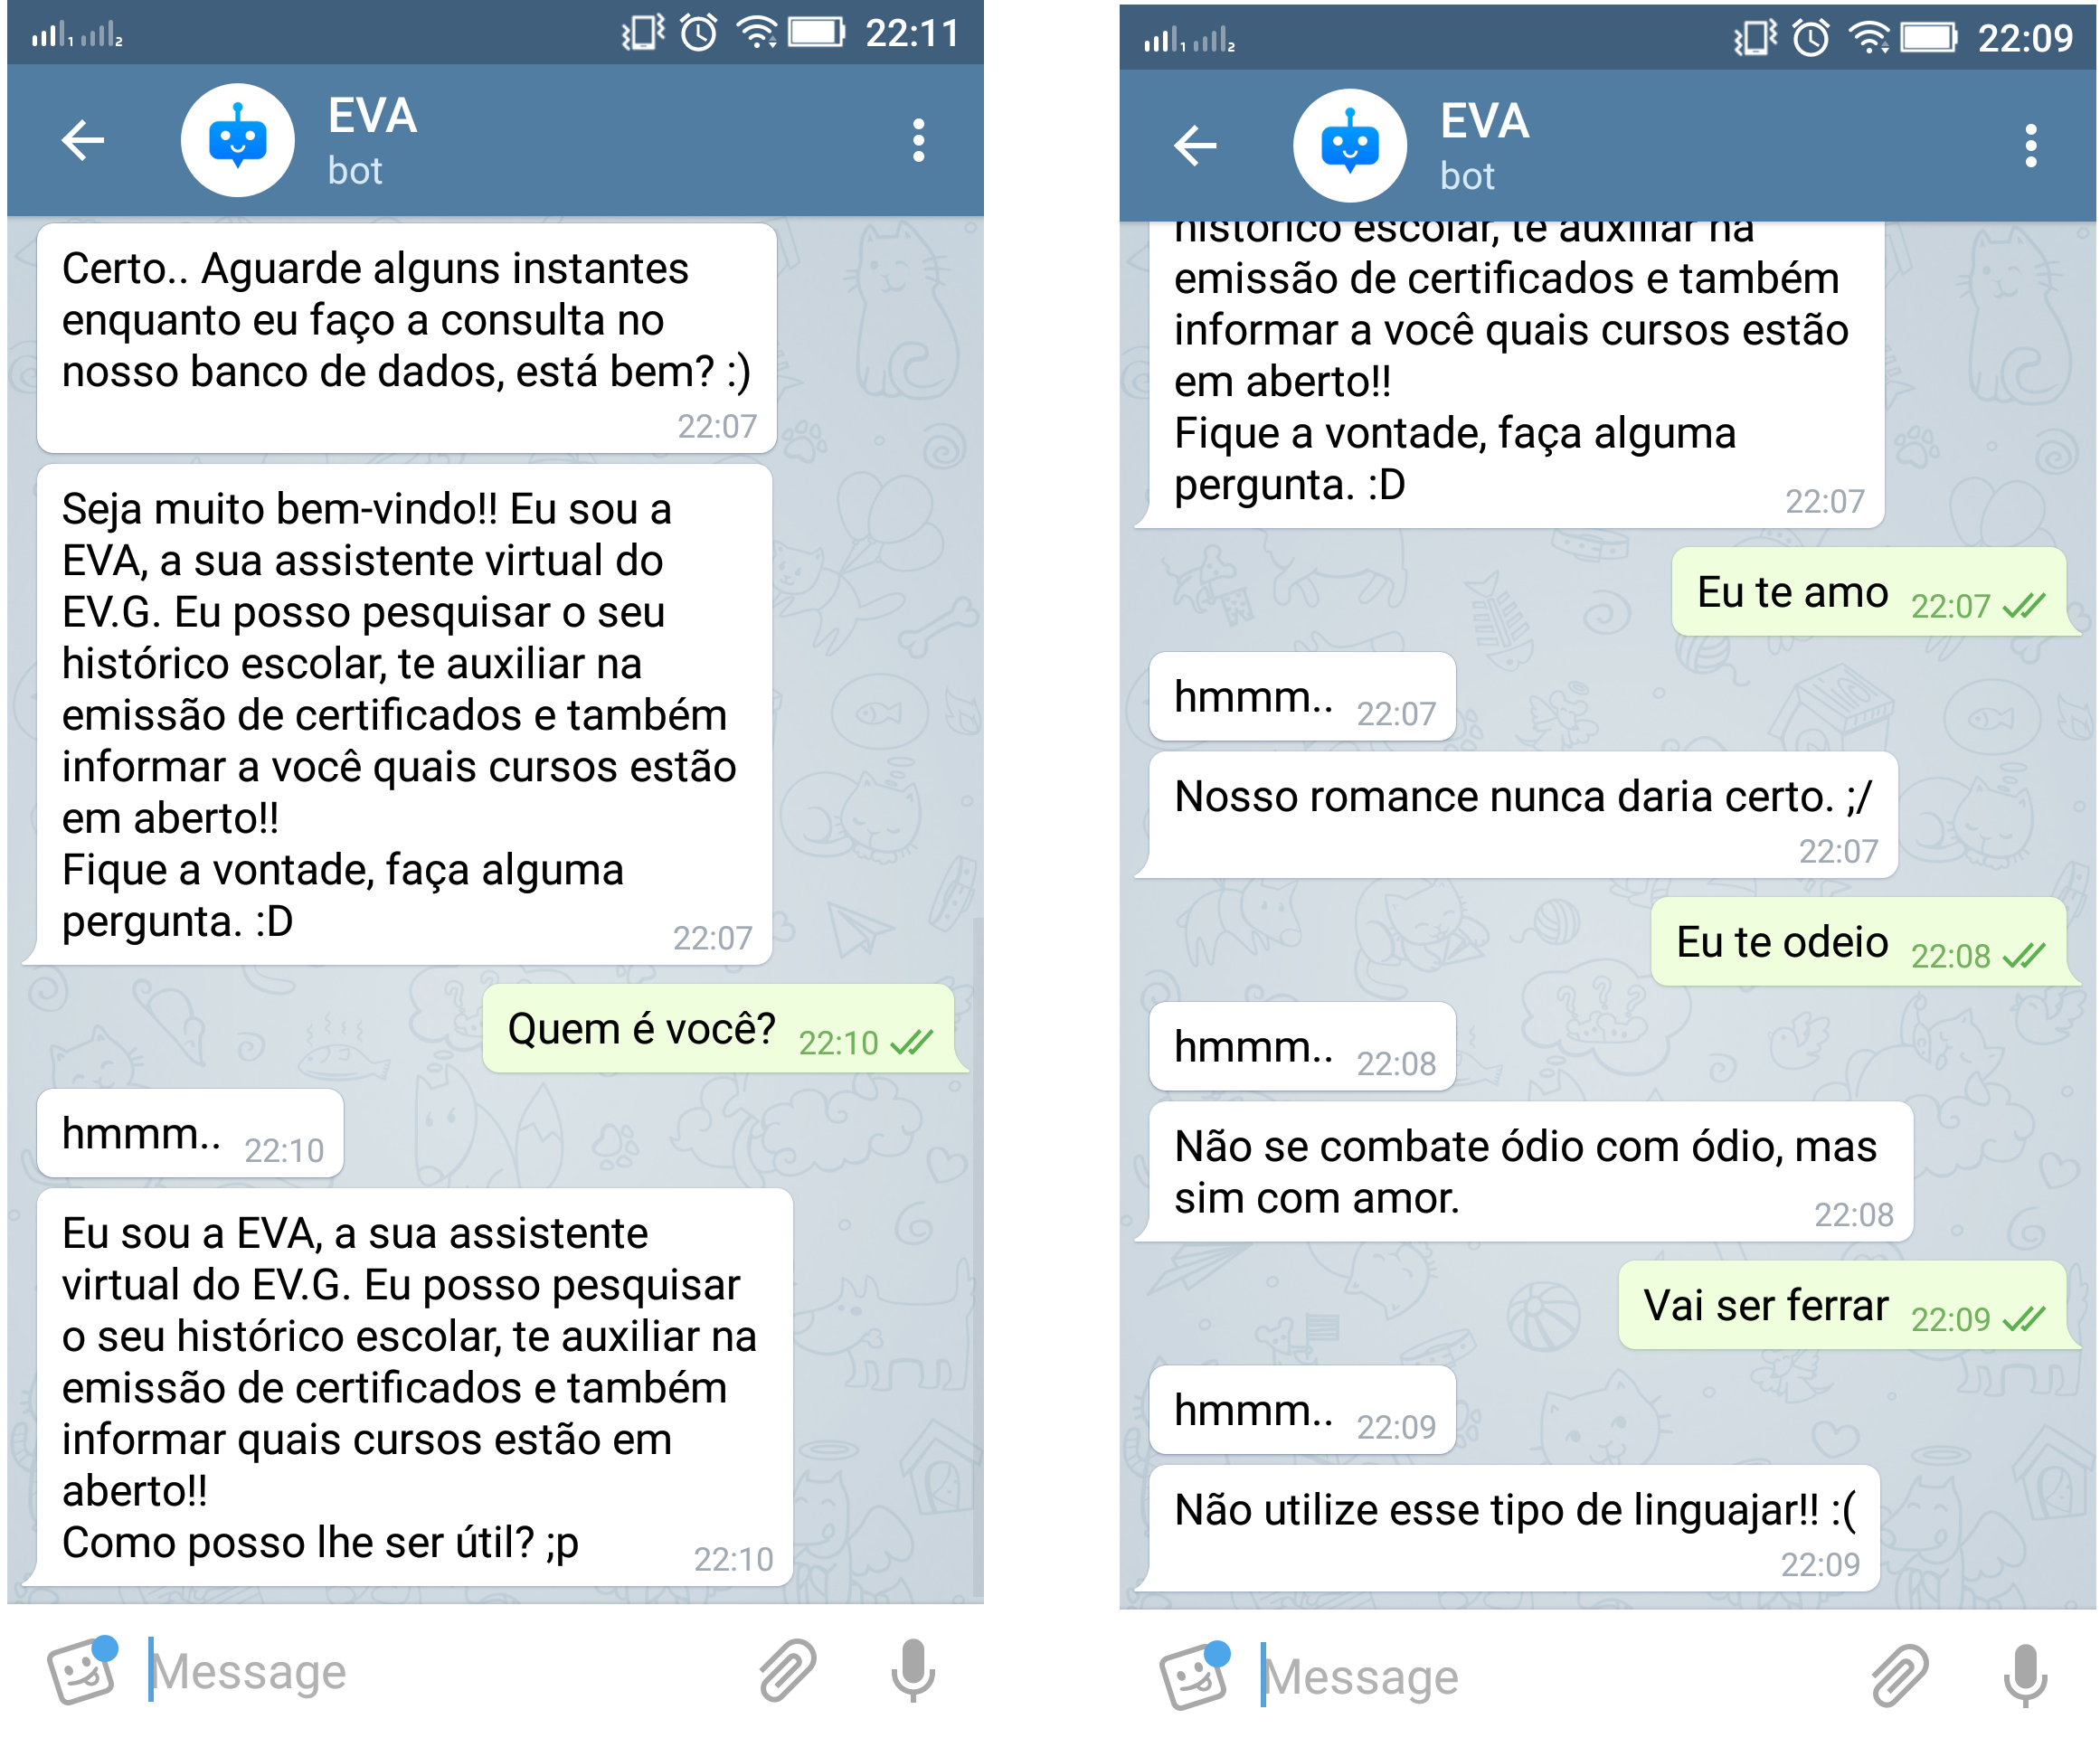
\includegraphics[width=0.4\linewidth]{imagens/apresentacao-dialogos.png}
  \mfonte
\end{figure}

\section{Visualizando o histórico escolar completo}

O aluno pode consultar o seu histórico escolar completo de maneira rápida e prática, como apresentado na Figura \ref{cap:04:fig:apresentacao-visualizar-historico}.

\begin{figure}
  \caption{
    \label{cap:04:fig:apresentacao-visualizar-historico}
    EVA - Visualizando histórico escolar completo
  }
  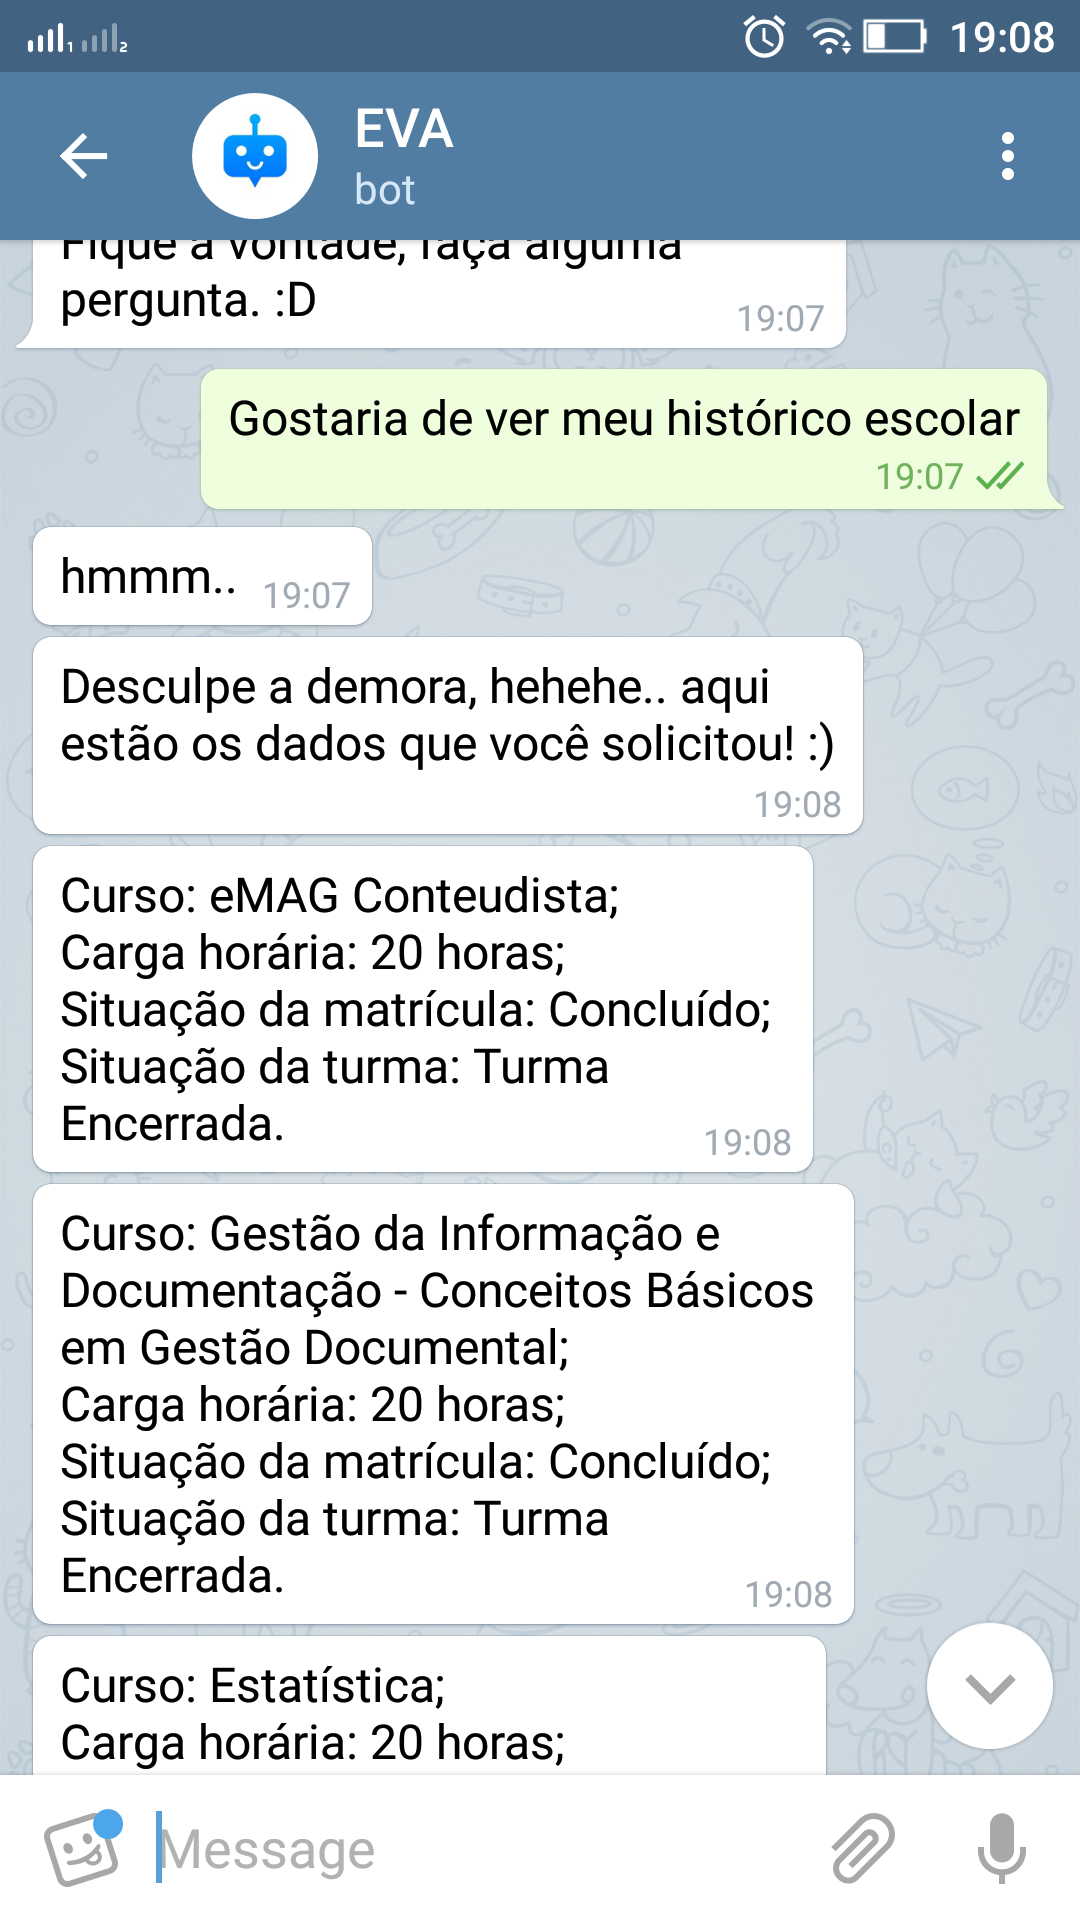
\includegraphics[width=0.2\linewidth]{imagens/apresentacao-visualizar-historico.png}
  \mfonte
\end{figure}

\section{Auxiliando na emissão de certificados}

Se o aluno desejar, EVA pode auxiliá-lo na emissão de certificados dos cursos concluídos por ele, como exibido na Figura \ref{cap:04:fig:apresentacao-auxilio-certificados}.

\begin{figure}
  \caption{
    \label{cap:04:fig:apresentacao-auxilio-certificados}
    EVA - Auxiliando na emissão de certificados
  }
  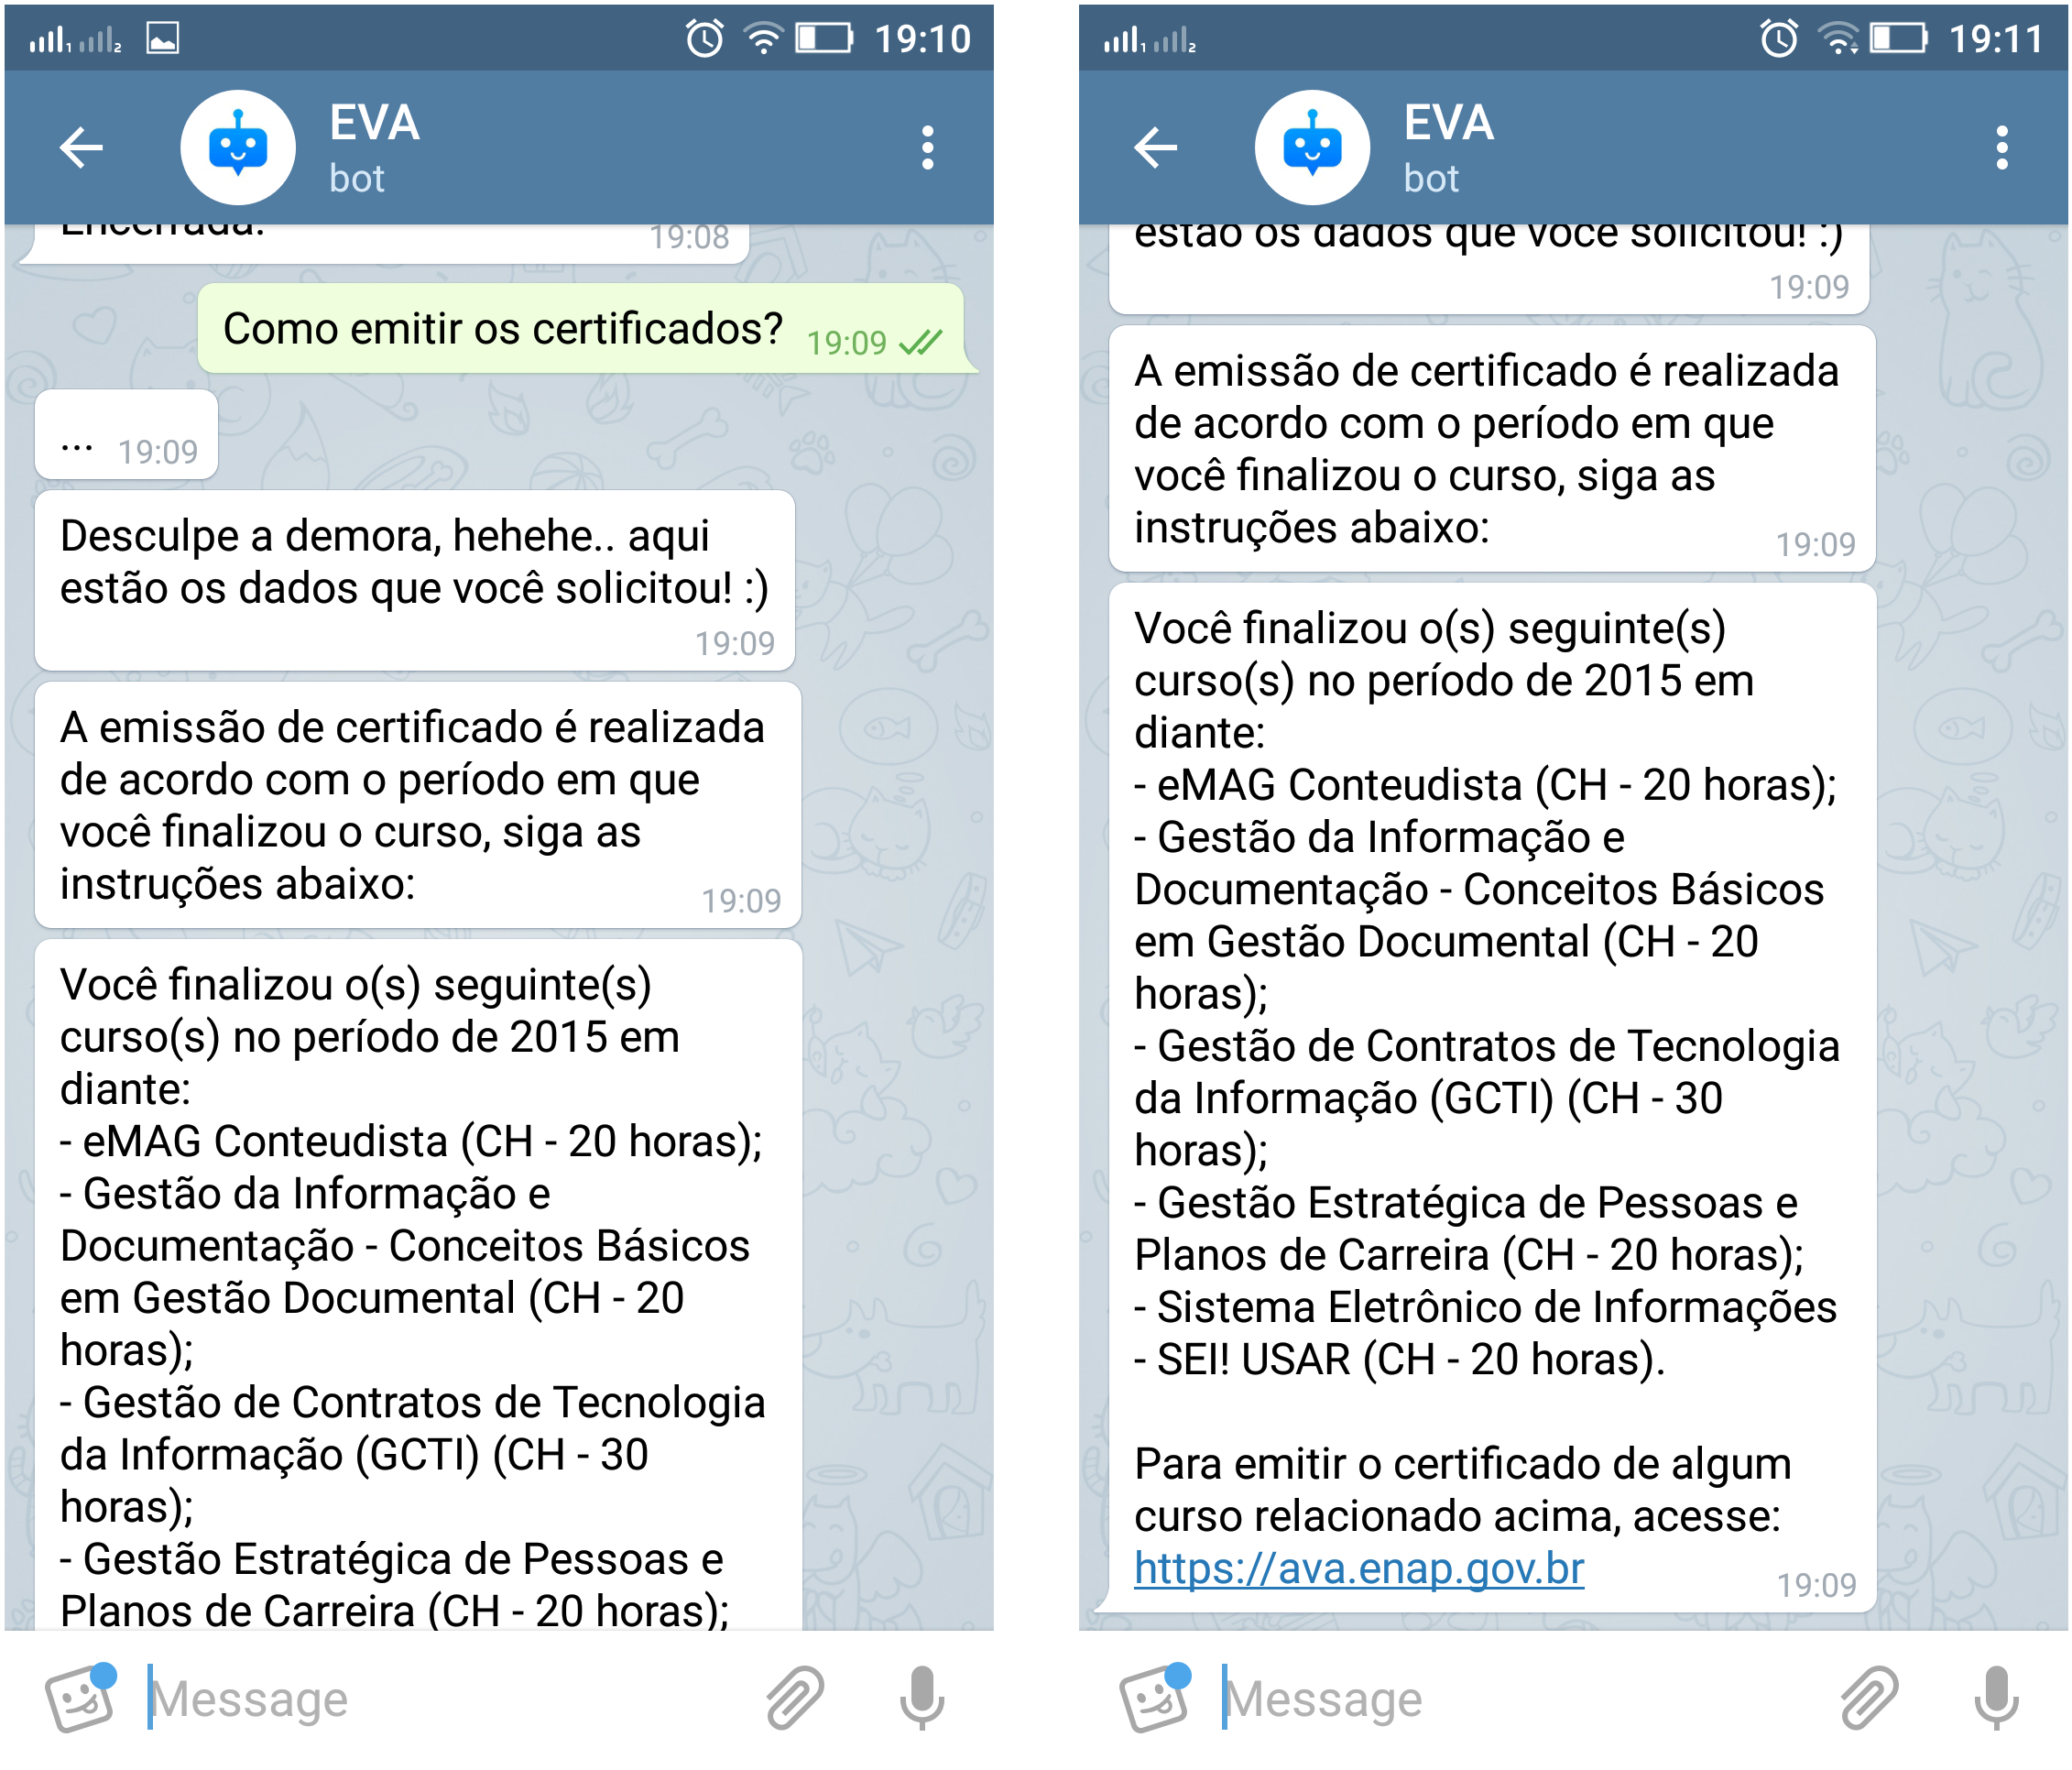
\includegraphics[width=0.4\linewidth]{imagens/apresentacao-auxilio-certificados.png}
  \mfonte
\end{figure}

\section{Visualizando inscrições de cursos em aberto}

Caso o aluno esteja em dúvida sobre quais inscrições de cursos estão em aberto, com uma mensagem de texto ele terá acesso a essas informações, como apresentado na Figura \ref{cap:04:fig:apresentacao-inscricoes-aberto}.

\begin{figure}
  \caption{
    \label{cap:04:fig:apresentacao-inscricoes-aberto}
    EVA - Visualizando inscrições de cursos em aberto
  }
  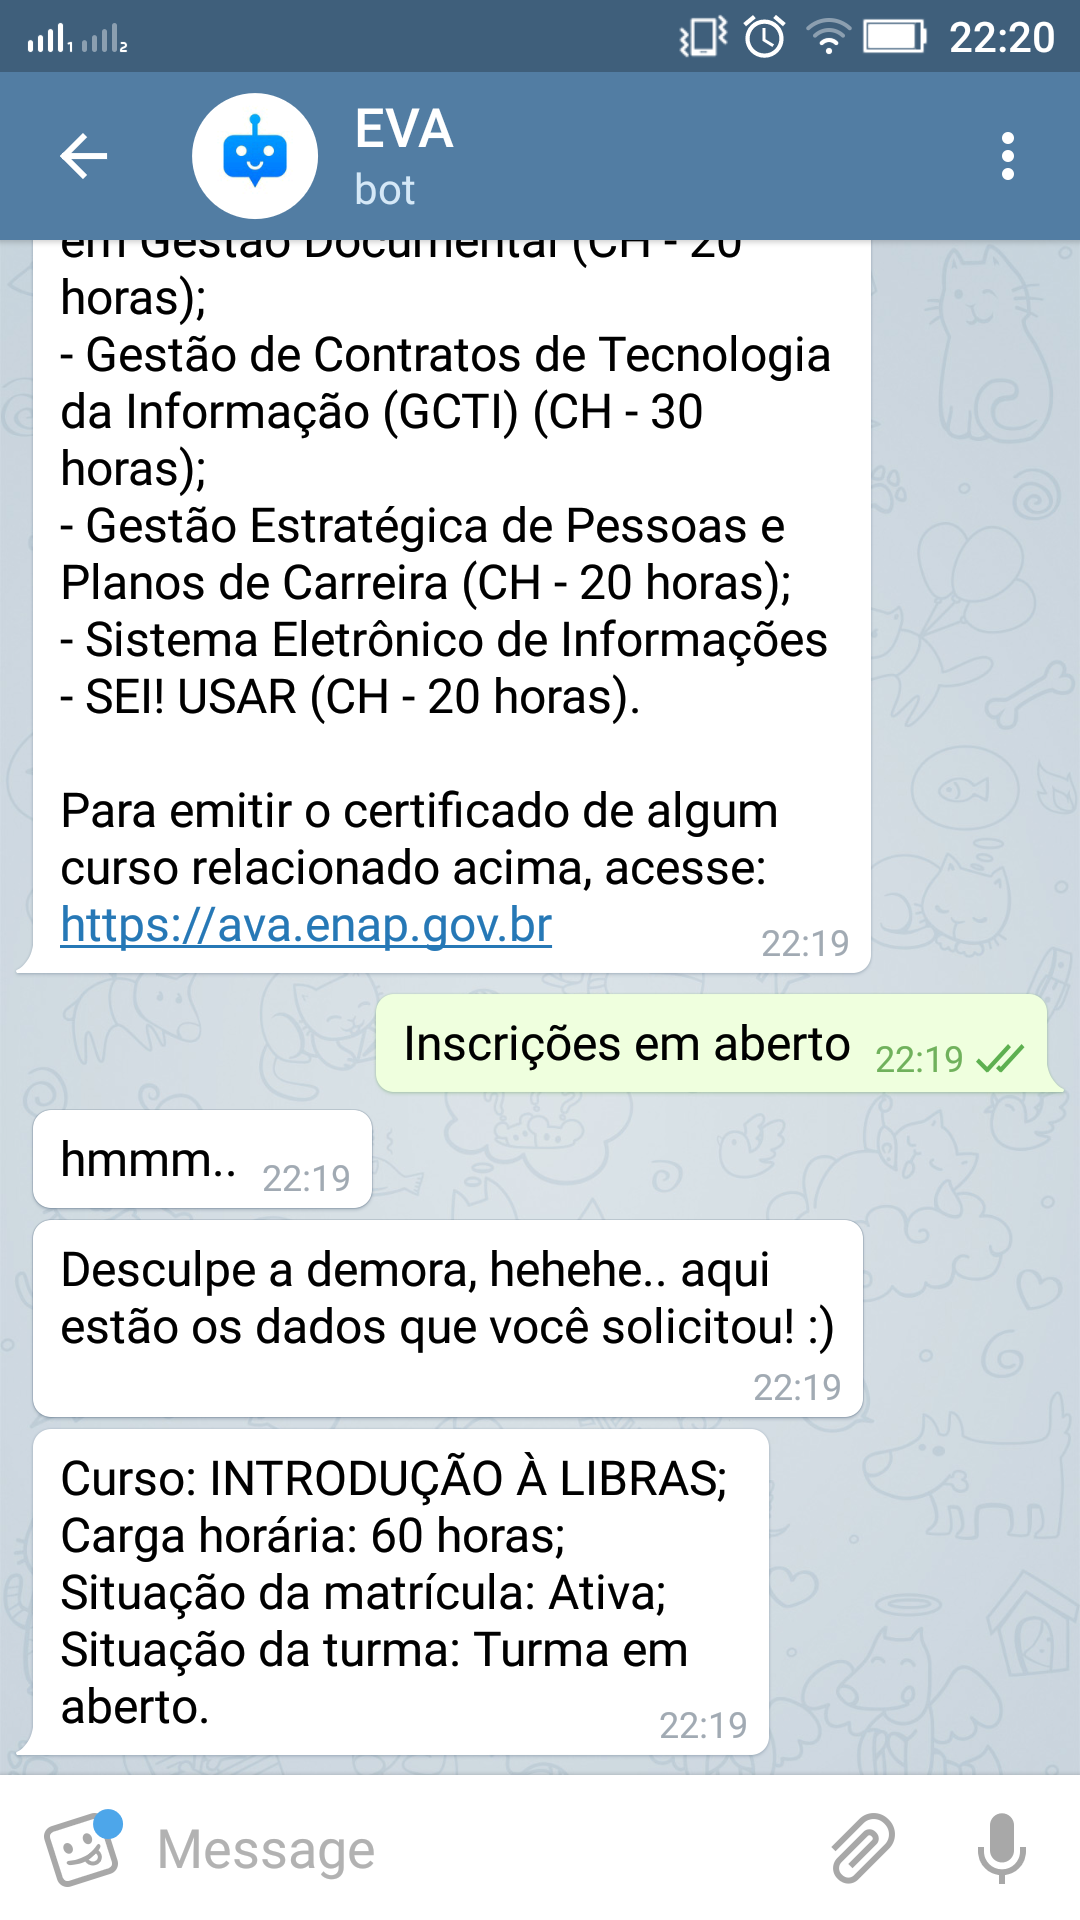
\includegraphics[width=0.2\linewidth]{imagens/apresentacao-cursos-aberto.png}
  \mfonte
\end{figure}

\section{Desvinculando}

A qualquer momento, se for da vontade do aluno, ele poderá se desvincular do sistema de EVA, apenas enviando uma simples mensagem de texto, demonstrado na Figura \ref{cap:04:fig:apresentacao-logout}.

\begin{figure}
  \caption{
    \label{cap:04:fig:apresentacao-logout}
    EVA - Logout
  }
  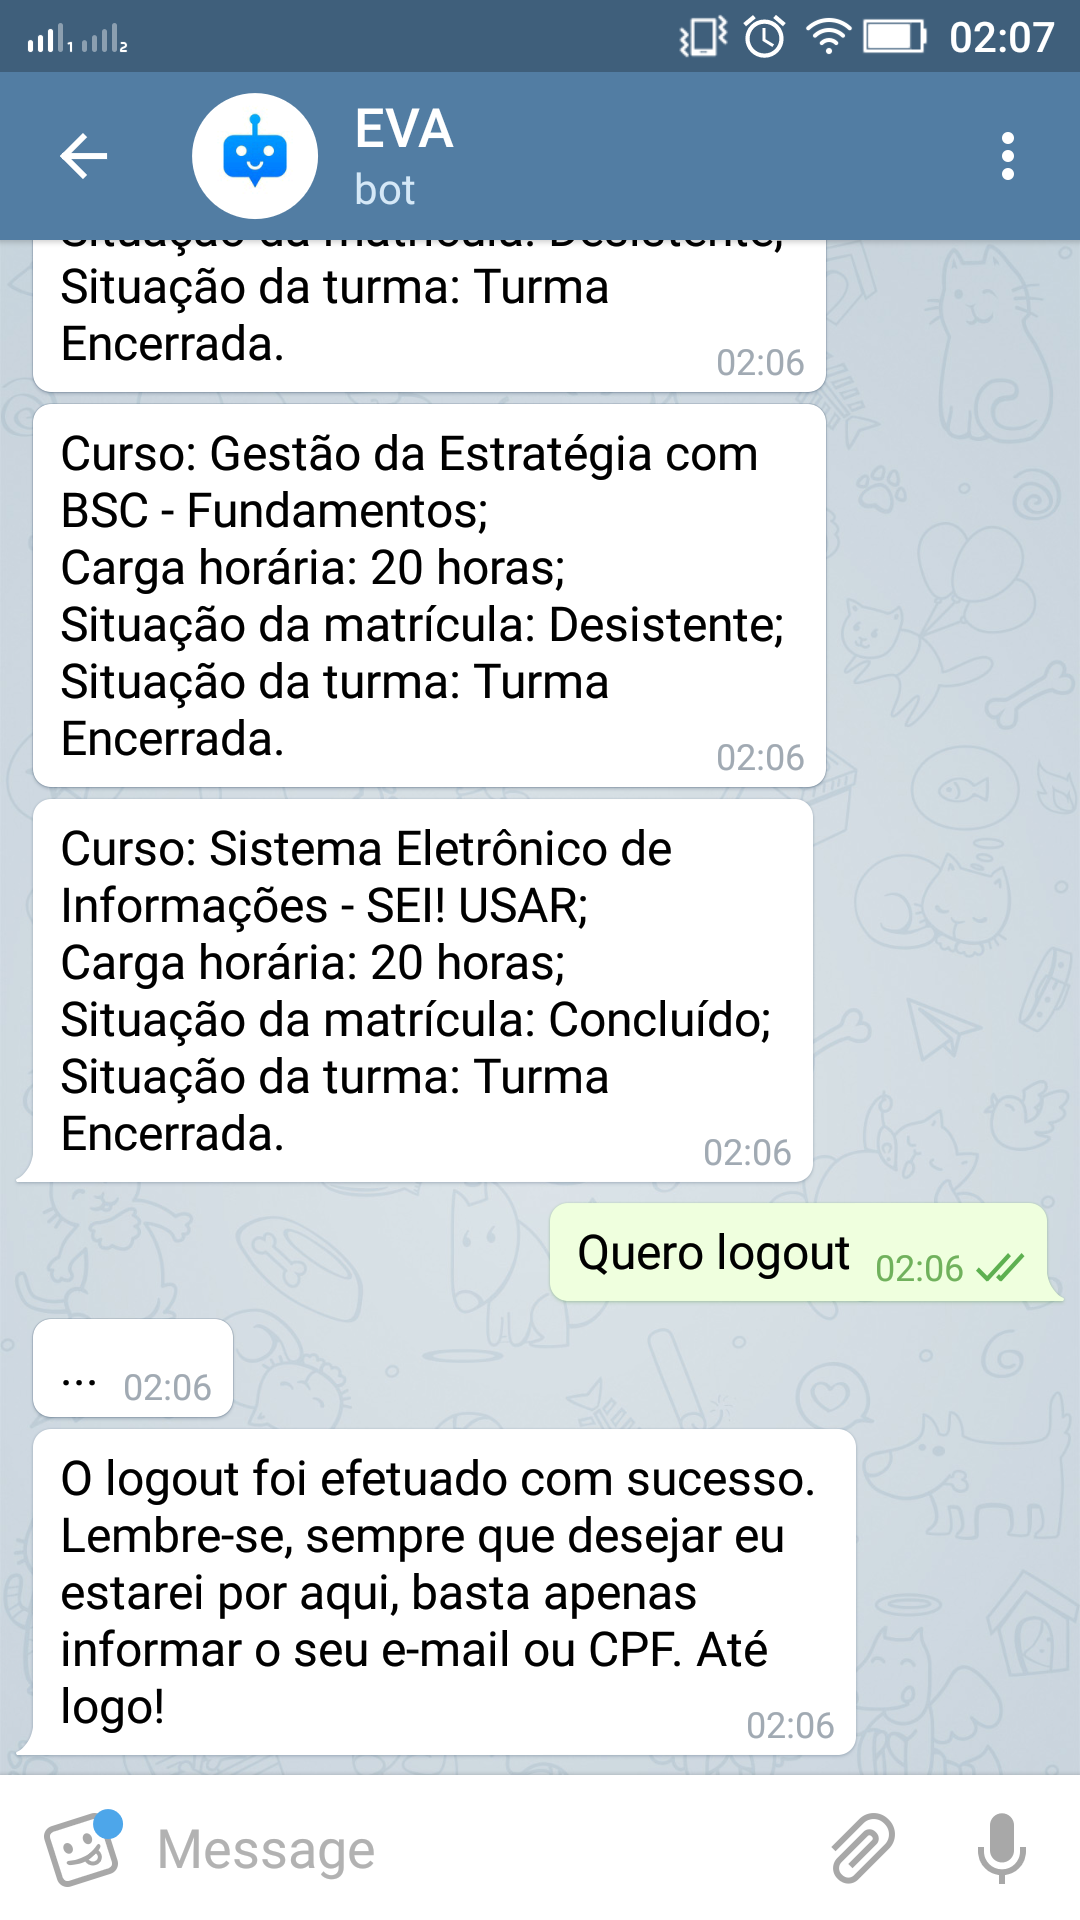
\includegraphics[width=0.2\linewidth]{imagens/apresentacao-logout.png}
  \mfonte
\end{figure}

  % Capitulo 5: Quinto capítulo (arquivo Includes/Capitulo5.tex)
  % MIT License
%
% Copyright (c) 2018 José Nascimento <joseaugustodearaujonascimento@gmail.com>
%
% Permission is hereby granted, free of charge, to any person obtaining a copy
% of this software and associated documentation files (the "Software"), to deal
% in the Software without restriction, including without limitation the rights
% to use, copy, modify, merge, publish, distribute, sublicense, and/or sell
% copies of the Software, and to permit persons to whom the Software is
% furnished to do so, subject to the following conditions:
%
% The above copyright notice and this permission notice shall be included in all
% copies or substantial portions of the Software.
%
% THE SOFTWARE IS PROVIDED "AS IS", WITHOUT WARRANTY OF ANY KIND, EXPRESS OR
% IMPLIED, INCLUDING BUT NOT LIMITED TO THE WARRANTIES OF MERCHANTABILITY,
% FITNESS FOR A PARTICULAR PURPOSE AND NONINFRINGEMENT. IN NO EVENT SHALL THE
% AUTHORS OR COPYRIGHT HOLDERS BE LIABLE FOR ANY CLAIM, DAMAGES OR OTHER
% LIABILITY, WHETHER IN AN ACTION OF CONTRACT, TORT OR OTHERWISE, ARISING FROM,
% OUT OF OR IN CONNECTION WITH THE SOFTWARE OR THE USE OR OTHER DEALINGS IN THE
% SOFTWARE.

% Considera��es finais
\chapter{Considerações finais}

Oferecer um serviço massivo sem a devida capacidade de atendimento aos usuários representa um risco para a qualidade e a sustentabilidade do serviço prestado. De um lado, tem-se a insatisfação dos usuários causada pela falta de atendimento, e, de outro, a incapacidade do provedor de colher informações que são estratégicas para a melhoria contínua dos serviços e para a tomada de decisão.

No âmbito da EV.G, observa-se que grande parte das solicitações dos alunos referem-se a assuntos simples, repetitivos e facilmente resolvidos a partir de uma consulta a informações disponíveis em banco de dados. É o caso de dúvidas relativas à emissão de certificados, procedimentos de inscrição, credenciais de acesso, entre outros. Dúvidas qualitativas, referentes à conteúdos, situações inéditas, por exemplo, são raras e podem ser direcionadas para um atendimento de segundo nível.  

Com o avanço tecnológico, soluções inovadoras e de baixo custo estão surgindo a todo momento. No cenário do atendimento on-line, o uso de \textit{chatbots} é uma opção de baixo custo e alto desempenho. Como tal, o \textit{chatbot} é uma solução possível para atendimento massificado via algum método de conversação, como por exemplo em aplicações de mensagens instantâneas.

No contexto da EV.G, foi desenvolvido um \textit{chatbot} de conversação textual compatível com a plataforma mensagens instantâneas chamada Telegram, denominado EVA (EV.G Virtual Assistant). O objetivo geral de EVA é automatizar a interação via texto no atendimento administrativo de primeiro nível a alunos no âmbito da secretaria acadêmica da EV.G.

EVA é um \textit{chatbot} de domínio amplo, que possui a capacidade de interagir com os alunos vinculados a EV.G na medida de suas necessidades. Em teoria, EVA não tem limite de atendimento simultâneo de alunos, nem tão pouco de horário de atendimento, por ser um programa de computador. O que torna ideal para atendimento em ambiente virtual de aprendizagem de alta disponibilidade, que é o caso da EV.G.

Por se tratar de um \textit{chatbot} de domínio amplo, EVA pode por meio de mecanismos de Inteligência Artificial, que para o seu caso utilizasse do PNL, aprender a partir das interações com os alunos e com isso, melhorar o seu repertório.



\section{Limitações}

O entendimento de EVA ainda é limitado devido ao seu pouco treinamento com base nas interações com os usuários do sistema, e também, devido as poucas intenções cadastradas e compreendidas durante a análise léxica, utilizando o PNL do Wit.ai. É válido ressaltar, que o Wit.ai oferece serviços para treinamento dos PNL desenvolvidos em sua plataforma, porém, devido ao escopo do presente trabalho, o treinamento realizado foi limitado às funcionalidades prioritárias requeridas pela EV.G.



\section{Trabalhos futuros}

Inicialmente, como primeira proposta de trabalhos futuros, seria a implantação do sistema de EVA em algum servidor. Buscando, por exemplo, maneiras eficiêntes para o armazenamento e também para o processamento do sistema.

Um dos intuitos da criação da API de EVA, se deu justamente para facilitar que o sistema possa continuar crescendo, podendo este atender em outras plataformas de mensagens instantâneas, tais como Facebook messenger ou até mesmo na própria plataforma da EV.G, permitindo aos alunos escolherem aquelas que melhor se adequem a suas realidades.

No que se diz respeito à usabilidade de EVA, poderá ser feito algum estudo sobre a experiência do usuário durante a interação com ela, com o intuito de melhorar ainda mais no atendimento aos alunos vinculados a EV.G. 

Poderão ser desenvolvidas novas funcionalidades que facilitem a modificação e adição de intenções compreendidas por EVA, e também, no que diz respeito ao seu repertório de respostas ao usuário. De modo a permitir que pessoas sem o conhecimento de programação de computadores, possam estar ajudando na expansão e nas melhorias de EVA.

Existe também um anseio por parte da EV.G de que as funcionalidades de EVA possam continuar a serem desenvolvidas, de modo que futuramente EVA possa ajudar proativamente na tutoria dos cursos oferecidos na plataforma. 

  % Consideracoes finais
  %% MIT License
%
% Copyright (c) 2018 José Nascimento <joseaugustodearaujonascimento@gmail.com>
%
% Permission is hereby granted, free of charge, to any person obtaining a copy
% of this software and associated documentation files (the "Software"), to deal
% in the Software without restriction, including without limitation the rights
% to use, copy, modify, merge, publish, distribute, sublicense, and/or sell
% copies of the Software, and to permit persons to whom the Software is
% furnished to do so, subject to the following conditions:
%
% The above copyright notice and this permission notice shall be included in all
% copies or substantial portions of the Software.
%
% THE SOFTWARE IS PROVIDED "AS IS", WITHOUT WARRANTY OF ANY KIND, EXPRESS OR
% IMPLIED, INCLUDING BUT NOT LIMITED TO THE WARRANTIES OF MERCHANTABILITY,
% FITNESS FOR A PARTICULAR PURPOSE AND NONINFRINGEMENT. IN NO EVENT SHALL THE
% AUTHORS OR COPYRIGHT HOLDERS BE LIABLE FOR ANY CLAIM, DAMAGES OR OTHER
% LIABILITY, WHETHER IN AN ACTION OF CONTRACT, TORT OR OTHERWISE, ARISING FROM,
% OUT OF OR IN CONNECTION WITH THE SOFTWARE OR THE USE OR OTHER DEALINGS IN THE
% SOFTWARE.

\anchor{chapter:chap6}
\chapter{Considerações finais}
\label{chapter:chap6}

À luz do presente trabalho, \dots

\section{Principais contribuições}

As principais contribuições do presente trabalho residem em:

\begin{enumerate}[label=\alph*)]
  \tightlist
  \item contribuição i;
  \item contribuição ii;
  \item \dots
\end{enumerate}

\anchor{consideracoes-finais--limitacoes}
\section{Limitações}

As limitações do presente trabalho são \dots

\section{Trabalhos futuros}

Limitações do trabalho, são:

\begin{enumerate}[label=\alph*)]
\tightlist
\item limitação i;
\item limitação ii;
\item \dots
\end{enumerate}
%--

  \backmatter

  % Bibliografia (arquivo Capitulos/Referencias.bib)
  %\nocite{*}
  \postextual
  \bibliography{referencias}
  %\bibliographystyle{abnt-alf}

  % Apêndice A (arquivo Includes/ApendiceA)
  %\begin{apendicesenv}
    %\partapendices

 %   % MIT License
%
% Copyright (c) 2018 José Nascimento <joseaugustodearaujonascimento@gmail.com>
%
% Permission is hereby granted, free of charge, to any person obtaining a copy
% of this software and associated documentation files (the "Software"), to deal
% in the Software without restriction, including without limitation the rights
% to use, copy, modify, merge, publish, distribute, sublicense, and/or sell
% copies of the Software, and to permit persons to whom the Software is
% furnished to do so, subject to the following conditions:
%
% The above copyright notice and this permission notice shall be included in all
% copies or substantial portions of the Software.
%
% THE SOFTWARE IS PROVIDED "AS IS", WITHOUT WARRANTY OF ANY KIND, EXPRESS OR
% IMPLIED, INCLUDING BUT NOT LIMITED TO THE WARRANTIES OF MERCHANTABILITY,
% FITNESS FOR A PARTICULAR PURPOSE AND NONINFRINGEMENT. IN NO EVENT SHALL THE
% AUTHORS OR COPYRIGHT HOLDERS BE LIABLE FOR ANY CLAIM, DAMAGES OR OTHER
% LIABILITY, WHETHER IN AN ACTION OF CONTRACT, TORT OR OTHERWISE, ARISING FROM,
% OUT OF OR IN CONNECTION WITH THE SOFTWARE OR THE USE OR OTHER DEALINGS IN THE
% SOFTWARE.

\chapter{Exemplo de apêndice}
\anchor{appendix:logo-ifrn}

\begin{figure}
  \centering
  
\includegraphics{logo-ifrn}
\end{figure}
%--
 %\end{apendicesenv}

  % Anexo A (arquivo Includes/AnexoA)
%   \begin{anexosenv}
%     \partanexos
%     \include{capitulos/AnexoA}
%   \end{anexosenv}

\phantompart
\printindex

\end{document}
%--